\documentclass[10pt,a4paper]{article}
\usepackage[utf8]{inputenc}
\usepackage[german]{babel}
\usepackage[T1]{fontenc}
\usepackage{amsmath}
\usepackage{amsfonts}
\usepackage{amssymb}
\usepackage[standard]{ntheorem}                            % Theorem-Umgebung
\usepackage{enumitem}
\usepackage{tikz}
\usepackage{extarrows}
\usepackage{physics}
\usepackage{todonotes}
\usepackage{csquotes}

\usepackage{hyperref}	%should be loaded last
\hypersetup{%
	unicode=true,%
	pdftitle=Analysis 2 MLG,%
	pdfauthor=Merle Gänssinger,%
	pdfkeywords=Analysis Lehramt,%
	pdfsubject=Skript zur Vorlesung Analysis 2 für Lehramtsstudenten für das Gymnasium,%
	pdflang=DE%
}


% Befehle um die Integrale angenehmer zu schreiben
\newcommand{\obint}[4][x]{\overline{\int_{#2}^{#3}} #4 \dd{#1}}
\newcommand{\unint}[4][x]{\underline{\int_{#2}^{#3}} #4 \dd{#1}}
% Verwendung:
% Optionales Argument mit [x]
% 1. Argument untere Grenze
% 2. Argument obere Grenze
% 3. Argument Funktion, die zu integrieren ist
% Beispiel mit Integration nach dy: \unint[y]{a}{b}{f(y)}
% oder kurz \unint[y] ab {f(y)}
\newcommand{\riemann}[2]{\mathcal{R}_{[{#1},{#2}]}}
% \riemann{1}{2} = \mathcal{R}_{[a,b]}

\begin{document}
%!TEX root = ../gesamt.tex

\section{Differentiation}
\begin{Definition}{
	Sei $f: D \left( f \right) \subseteq \mathbb{R} \rightarrow \mathbb{R}$ 
	und $x_0 \in D \left( f \right)$ ein Punkt, 
	um den ein offenes Intervall $B_{\epsilon} \left( x \right)$ 
	(für geeignetes $\epsilon > 0$) komplett 
	in $D \left( f \right)$ enthalten ist $\left( B_{\epsilon} \left( x \right)
	 \subseteq D \left( f \right) \right) $. Dann heißt $f$ an der Stelle $x_0$ 
	 \emph{differenzierbar}, wenn der Grenzwert
	\begin{equation*}
		Df\left(x_0\right) := \frac{df}{dx} 
		\left( x_0 \right) := f'\left( x_0 \right) 
	\end{equation*}
	\begin{equation*}
	\lim\limits_{x \rightarrow x_0}{\frac{f 
	\left( x \right) - f \left( x_0 \right) }{x - x_0} }
	\end{equation*} 
	existiert. \\
	Wir meinen mit $f'\left(x_0\right)$ die \emph{Ableitung} 
	(seltener \emph{Differentialquotient}) von $f$ an der Stelle $x_0$. \\
	Ist $f: D\left(f \right) \rightarrow \mathbb{R}$ in jedem $x \in D\left(f\right)
	$ differenzierbar, dann heißt $f$ schlechthin \emph{differenzierbar}. 
	Etwas irreführend wird auch die Abbildung  
	\begin{equation*}
		f': D\left(f\right) \subseteq \mathbb{R} \rightarrow \mathbb{R}
	\end{equation*}
	\begin{equation*}
		x \mapsto f'(x)
	\end{equation*}
	als Ableitung von $f$ bezeichnet.
}\end{Definition}

\begin{Satz}{
	Sei $I \subseteq \mathbb{R}$ ein offenes Intervall und $f: I \rightarrow \mathbb{R}$ und $x_0 \in I$. Dann sind äquivalent:
	\begin{enumerate}
		\item \label{satz1:i}Es gibt ein $c \in \mathbb{R}$ und $\phi: I \rightarrow \mathbb{R}$, so dass
		\begin{equation*}
		f\left(x\right) = f\left(x_0\right) + c\left(x-x_0\right) + \phi\left(x\right)
		\end{equation*} 
		und 
		\begin{align} 
			\lim\limits_{x \rightarrow x_0}{\frac{\phi\left(x\right)}{x-x_0}}  = 0
			\label{gleichung:i}
		\end{align}
		\item Es gibt ein $ \tilde{c} \in \mathbb{R}$ und $
		u: I \rightarrow \mathbb{R}$, so dass 
	\begin{equation*}		
		f\left(x\right) = f\left(x_0\right) + \tilde{c}\left(x-x_0\right) + u\left(x
		\right)\left(x-x_0\right)
		\end{equation*}
		und 
		\begin{equation*}
		\lim\limits_{x \rightarrow x_0}{u\left(x\right) = 0}
		\end{equation*}
		\item $f$ ist in $x_0$ differenzierbar
	\end{enumerate}
	Gelten die obigen Aussagen, so gilt 
	\begin{equation*}
		f''\left(x_0\right) = c = \tilde{c}
	\end{equation*}
	Das heißt insbesondere $c$ und $\tilde{c}$ sind eindeutig bestimmt

}\end{Satz}

\begin{Bemerkung}{
	\begin{itemize}
		\item[ ]
		\item Der springende Punkt in \ref{gleichung:i} ist 
		Gleichung~\ref{gleichung:i}. Ohne Gleichung~\ref{gleichung:i} 
		kann man sich ein beliebiges $c \in \mathbb{R}$ wählen und setzt 
	\begin{equation*}
	\phi\left(x\right) := f\left(x\right) - f\left(x_0\right) - c\left(x-x_0\right)
	\end{equation*}			
	\item Vergisst man die Funktion $\phi$, versteht man mit der Geradengleichung \todo{Hier ist der Satz unvollständig}
		\begin{equation*}
		x \mapsto f\left(x_0\right) + c\left(x-x_0\right)
		\end{equation*}
		Das ist per Definition die Gleichung der Tangente an $f$ in $x_0$
	\end{itemize}
}\end{Bemerkung}

\begin{proof}{
	\begin{itemize}
		\item[ ]
		\item[]$1 \leftrightarrow 2$ Man setzte einfach $u\left(x\right) = \frac{\phi\left(x\right)}{x-x_0}$ und $\tilde{c} = c$ \\
		(in $x = x_0$ setze man $u\left(x_0\right) = 0$)
		\item[]$1 \rightarrow 2$ ZZ $\lim\limits_{x \rightarrow x_0}{\frac{f\left(x\right)-f\left(x_0\right)}{x-x_0}}$ existiert
		\begin{align*}
			\lim\limits_{x\rightarrow x_0}
			{\frac{f\left(x\right) - f\left(x_0\right)}{x-x_0}} 
			= & \lim\limits_{x \rightarrow x_0}
			{\frac{f\left(x_0\right) + c\left(x-x_0\right)+\phi
			\left(x\right)-f\left(x_0\right)}{x-x_0}} \\
			 = & \lim\limits_{x\rightarrow x_0}
			{c + \frac{\phi \left(x\right)}{x-x_0}} = c
		\end{align*}
		\item[]$3\rightarrow 1$ Wir setzten $ c = f'\left(x_0\right)$ und 
		\begin{equation*}
			\phi\left(x\right) = f\left(x\right) - f\left(x_0\right) - f'\left(x_0\right)\left(x-x_0\right)
		\end{equation*}
		offensichtlich gilt dann:
		\begin{equation*}
			f\left(x\right) = f\left(x_0\right) 
			+ f'\left(x_0\right)\left(x-x_0\right) + \phi\left(x\right)
		\end{equation*}
		\begin{align*}
			\lim\limits_{x\rightarrow x_0}
			{\left\vert \frac{\phi\left(x\right)}{x-x_0}\right\vert} 
			= & \lim\limits_{x \rightarrow x_0}
			{\left\vert \frac{f\left(x\right)-f\left(x_0\right)-
			f'\left(x_0\right)\left(x-x_0\right)}{x-x_0}\right\vert} \\
			= & \lim\limits_{x\rightarrow x_0}{\frac{f\left(x\right)-
			f\left(x_0\right)}{x-x_0} - f'\left(x_0\right)} \\
			= & f'\left(x_0\right) - f\left(x_0\right) 
			=0
		\end{align*}
	\end{itemize}
	\qedhere
}\end{proof}

\setcounter{Satz}{1} 
\setcounter{Definition}{5}

\begin{Satz}{
	Es sind äquivalent: $f : I \rightarrow \mathbb{R}$
	\begin{enumerate}
		\item $f(x) = f(x_0) + f'(x_0) \cdot (x-x_0) + \phi(x) $\\
		 mit: $\lim\limits_{n \rightarrow \infty}{\frac{\phi(x)}{|x-x_0|}} = 0$
	\item $ f(x) = f(x_0) + f'(x_0) \cdot (x-x_0) + \phi(x) + u(x)  \cdot (x-x_0)$ \\
	mit: $\lim\limits_{n \rightarrow \infty}{u(x)} = 0$
	\item Der Grenzwert 
	$f'(x_0) = \lim\limits_{n \rightarrow \infty}{\frac{f(x)-f(x_0)}{x-x_0}}$ 	
	existiert
	\end{enumerate}
}\end{Satz}

\begin{Satz}{\label{satz:satz_3}
	Sei $ I \subseteq \mathbb{R}$ ein Intervall, $f: I \rightarrow \mathbb{R}$ 
	differenzierbar in $x_0 \in I$. Dann ist f in $x_0$ stetig. \\
	\textbf{Beweis:} \\
		\noindent\hspace*{5mm}
		\textit{ZZ}  ist: $\lim\limits_{x \rightarrow x_0}{f(x) = f(x_0)}$ \\
		\noindent\hspace*{10mm}
		Äquivalent dazu: $\lim\limits_{x \rightarrow x_0}{f(x)-f(x_0) = 0}$. \\
		\noindent\hspace*{10mm}
		Nun gilt: $\lim\limits_{x \rightarrow x_0}{f(x) - f(x_0)} = 
	 \lim\limits_{x \rightarrow x_0}{\frac{f(x)-f(x_0)}{\frac{x-x_0}{x-x_0}}}
	 = f'(x_0) \cdot 0 = 0 $
}\end{Satz}
\begin{Bemerkung}{
	 \begin{itemize}
	 	\item[ ]
	 	\item Die Umkehrung dieser Aussage ist im Allgemeinen falsch! \\
	 	Es gibt sogar Funktionen, die überall stetig aber nirgends 
	 	differenzierbar sind. \\
	 	(\textit{Beispiel:} Weierhaus-Fkt: $\sum_{n \in \mathbb{N}} cos(b_n \pi x)$
	 	mit $a_n \in (0,1)$ und $a_n b_n >1$)
	 	\item Jede nicht stetige Funktion ist nicht differenzierbar
	 \end{itemize}	 
}\end{Bemerkung}

\begin{Satz}{
	Seien $f,g : I \rightarrow \mathbb{R}$ in $x \in I$ differenzierbar, 
	$ I \subseteq \mathbb{R}$ ein Intervall. Dann sind $f +g$, $f \cdot g$ und 
	$\frac{f}{g}$ (sofern $g(x) \neq 0 $)  in $x$ differenzierbar. \\
	Es gilt:
	\begin{enumerate}
		\item $(f + g)' = f'(x) + g'(x)$ (Summenregel)
		\item $(f \cdot g)' = f'(x)g(x) + f(x) \cdot g'(x) $ (Produktregel)
		\item $ (\frac{f}{g})' = \frac{f'(x)g(x) - f(x)g'(x)}{g^2(x)}$ 	
		(Quotientenregel) 
	\end{enumerate}
	\textbf{Beweis:}
	\begin{enumerate}
		\item $(f+g)'(x) = 
		\lim\limits_{y \rightarrow x}{\frac{f(y)+g(y) - (f(x) + g(x))}{y- x}} = 
		\lim\limits_{y \rightarrow x}{\frac{f(y) - f(x)}{y-x} + \frac{g(y) -g(x)}
		{y-x}}  \\ \noindent\hspace*{17mm}
		= \lim\limits_{y \rightarrow x}{\frac{f(y)-f(x)}{y-x}} + 
		\lim\limits_{y \rightarrow x}{\frac{g(y)-g(x)}{y-x}} 
		= f'(x) + g'(x)$
		
		\item $\lim\limits_{y \rightarrow x}{\frac{f(y)g(y) - f(x)g(x)}{y-x}} = 
		\lim\limits_{y \rightarrow x}{\frac{f(y)g(y) - f(y)g(x) 
		+ f(y)g(x)-f(x)g(x)}{y-x}} \\ \noindent\hspace*{17mm}
		= \lim\limits_{y \rightarrow x}{f(y) \frac{g(y)-g(x)}{y-x} + g(x) 
		\frac{f(x)-f(x)}{y-x}} \\ \noindent\hspace*{17mm}
		=\lim\limits_{y \rightarrow x}f(y) 
		\lim\limits_{y \rightarrow x}{\frac{g(y) - g(x)}{y-x}} + g(x) 
		\lim\limits_{y \rightarrow x}{\frac{f(y)-f(x)}{y-x}} 
		\\ \noindent\hspace*{17mm}
		\overset{Satz~\ref{satz:satz_3}}{=} f(x)g'(x) + g(x)f'(x)$
		
		\item $
		\lim\limits_{y \rightarrow x}
			{\frac{\frac{f(y)}{g(y)} - \frac{f(x)}{g(x)}}{y-x}}
		= \lim\limits_{y \rightarrow x}{\frac{\frac{f(y)}{g(y)}\frac{g(x)}{g(x)} -
			\frac{f(x)}{g(x)}\frac{g(y)}{g(y)}}{y-x}}
		= \lim\limits_{y \rightarrow 	x}{\frac{1}{g(y)g(x)} 
			\frac{f(y)g(x)-f(x)g(y)}{y-x}} \\ \noindent\hspace*{17mm}
		=\frac{1}{g^2(x)} \lim\limits_{y \rightarrow x}
			{\frac{f(y)g(x) -f(y)g(y) + f(y)g(y) -f(x)g(y)}{y-x}} 
		\\	\noindent\hspace*{17mm}
		= \frac{1}{g^2(x)} \lim\limits_{y \rightarrow x} 
		{f(y) \cdot \frac{g(x)-g(y)}{y-x} + g(y) \frac{f(y)-f(x)}{y-x}} 
		\\ \noindent\hspace*{17mm}
		= \frac{1}{g^2(x)} \cdot \left( \lim\limits_{y \rightarrow x}
			{f(y) \frac{g(x) - g(y)}{y-x}} + \lim\limits_{y \rightarrow x}
			{g(y) \frac{f(y) - f(x)}{y-x} } \right) \\ \noindent\hspace*{17mm}
		= \frac{1}{g^2(x)}(f(x)\cdot(-g(x)) + g(x)f'(x)) 
		= \frac{g(x)f'(x) - f(x)g'(x)}{g^2(x)}$
	\end{enumerate}	 
}\end{Satz}

\begin{Beispiel}{
	\begin{itemize}
	\item[]
		\item[•\label{punkt_1}]$f(x) = c \in \mathbb{R} (x \in \mathbb{R})$ \\
		$\rightarrow f'(x) = \lim\limits_{x \rightarrow y}{\frac{f(y)-f(x)}{y-x}}
		= \lim\limits_{x \rightarrow y}{\frac{c - c}{y-x}} = 0$
		
		\item[•\label{punkt_2}]  $f(x) = x (x \in \mathbb{R}) \\
		f'(x) = \lim\limits_{x \rightarrow y}{\frac{y-x}{y-x}} = 1$
		
		\item $f(x) = x^n, (x\in\mathbb{R})$ wobei $n \in \mathbb{N}$ \\
		$f'(x) = n x^{n-1}$ per Induktion: \\
		\noindent\hspace*{5mm} \textbf{$n = 1$} Stichpunkt 2 $\checkmark$ \\
		\noindent\hspace*{5mm} \textbf{$n \rightarrow n+1$}: 
		Sei also $f(x) = x^{n+1}$. Das gibt mit der Produktregel: \\
		\noindent\hspace*{5mm} $f'(x) = (x \cdot x^n)' = (x)' \cdot (x^n)' 
		= 1\cdot x	n + x \cdot n \cdot 
		x^{n-1} = x^n + nx^n = (n+1)x^n$
	\end{itemize}
}\end{Beispiel}

Damit sind alle Polynome differenzierbar und für 
$p(x) = \sum_{l=0}^{n} a_l x^l$ gilt (Summenregel):
\begin{equation*}p'(x) = \sum_{l = 0}^n l \cdot a_l \cdot x^{l-1} 
= \sum_{l=1}^n l \cdot a_l x^{l-1}
\end{equation*}

\begin{itemize}
	\item Seien $P_1$ und $P_2$ Polynome. \\
	Dann nennt man die Abbildung \\
	\noindent\hspace*{5mm}$Q : \mathbb{R}\setminus\{x|P_2(x) = 0\}
	\rightarrow \mathbb{R} \\
	\noindent\hspace*{6mm}x \mapsto \frac{P_1(x)}{P_2(x)}$ 
	eine rationale Funktion. \\
	Mit obiger sehen wir: rationale Funktionen sind auf dem kompletten
	 Definitionsbereich differenzierbar.
	 
	\item Die Funktion $|\circ | \cdot x \mapsto |x| = \begin{cases}x  & \textit{für } x\geq 0 \\ - x & sonst \end{cases}$
	ist nicht in 0 differenzierbar. Denn:
	\begin{equation*}
	\lim\limits_{y \searrow 0}{\frac{|y|-|0|}{y-0}}
	= \lim\limits_{y \searrow 0}{\frac{y-0}{y-0}} = 1 
	\end{equation*}
	\begin{equation*}
	\lim\limits_{y \nearrow 0}{\frac{|y| -|0|}{y-0}} = \lim\limits_{y 
	\nearrow 0}{\frac{-y-0}{y-0}} = -1
	\end{equation*}
\end{itemize}

\begin{Satz}[Kettenregel]{
	Seien $I_f$ und $I_g$ Intervalle, $x_0 \in I_f$ und 
	$f : I_f \rightarrow \mathbb{R}$ in $x_0$ differenzierbar und 
	$g: I_g \rightarrow \mathbb{R}$ sei in $f(x_0)$ differenzierbar und 
	$f(I_f) \subseteq I_g$. Dann gilt:
	\begin{equation*}
	\frac{d g \circ f}{dx}(x_0) = \frac{dg}{dx}(f(x_0)) \cdot \frac{df}{dx}(x_0)
	\end{equation*}
	
	\textbf{Beweis:}
	Da f in $x_0$ differenzierbar ist, gilt für alle 
	$x \in I_f$:
	\begin{equation*}
		f(x) -f(x_0) = (x-x_0) \cdot(f'(x_0) + u(x))
	\end{equation*}
	$($Wobei $\lim\limits_{x \rightarrow x_0}{u(x) = 0})$ \\
	Analog gilt für alle $y \in I_g$:
	\begin{equation*}
		g(y) -g(f(x_0)) = (y-f(x_0)) \cdot (g'(f(x_0)) + v(y)),
	\end{equation*}		
	\noindent\hspace*{5mm}wobei $\lim\limits_{y \rightarrow f(x_0)}{v(y) = 0}$ \\
	\noindent\hspace*{5mm}Damit haben wir für alle $x \in I_f$:
	\begin{align*}
	g(f(x)) - g(f(x_0)) = & (f(x)-f(x_0)) \cdot (g'(f(x_0)) + v(f(x)) \\
	= & (x-x_0)(f'(x_0) + u(x)) (g'(f(x_0)) + v(f(x))
	\end{align*}
	\noindent\hspace*{5mm}Damit gilt:
	\begin{align*}
	\lim\limits_{x \rightarrow x_0}
	{\frac{g(f(x))-g(f(x_0))}{x-x_0} } 
	= & \lim\limits_{x \rightarrow x_0}{(f'(x_0) + u(x)) (g'(f(x)) + v(f(x))} \\
	= & \lim\limits_{x \rightarrow x_0}{(f'(x_0) + u(x))} 
	\lim\limits_{x \rightarrow x_0}{(g'(f(x_0)) + v(f(x)))} \\
	= & (f'(x_0) + 0) (g'(f(x_0)) + 0)
	= f'(x_0) g'(f(x_0))
	\end{align*}
}\end{Satz}

\begin{Definition}{
	Ist $I \subseteq \mathbb{R}$ ein Intervall und 
	$f: I \rightarrow \mathbb{R}$ differenzierbar und $f':I \rightarrow \mathbb{R}$
	stetig. Dann heißt f \textbf{stetig differenzierbar}. 
	Wir definieren weiterhin induktiv die 
	k-te Ableitung (für $k \in \mathbb{N}$) durch:
	\begin{align*}
		f^{(0)} := & f \\
		f^{(k+1)} := & f^{(k+1)'}
	\end{align*}
	sofern die Ableitungen definiert sind.\\
	Ist $f^{(k)}: I \rightarrow \mathbb{R}$ für alle $k \in \mathbb{N}$ definiert, 
	so heißt f \textbf{beliebig oft} bzw. \textbf{unendlich oft differenzierbar}.
}\end{Definition}

\begin{Bemerkung}{Wir haben bereits gesehen: Polynome sind beliebig oft
	 differenzierbar.
}\end{Bemerkung}
\setcounter{Satz}{6} 
\begin{Satz}{
	Sei $p \left( x\right) = \sum_{k=0}^{ \infty}
	{ a_k \left( x-x_0\right)^k}, a_k \in 
	\mathbb{R} ,x_0 \in \mathbb{R}$ eine Potenzreihe vom Konvergenzradius 
	$R >0 $. Dann ist $p : x \mapsto p\left(x\right)$ auf ganz 
	$\left( x_0-R, x_0+R \right)$ differenzierbar mit 
	$p'\left( x \right) = \sum_{k=0}^\infty {\left( k+1\right) 
	a_{k+1} \left(x-x_0\right)^k}$.\\
	Insbesondere ist $p'$ auch wieder eine Potenzreihe 
	(die man durch gliedweises differenzieren erhält) mit	Konvergenzradius R.
}\end{Satz}

\begin{Bemerkung}{
	\begin{enumerate}
		\item[ ]
		\item Damit erhalten wir: 
		\begin{equation*}
			exp'\left(x\right) = \left( \sum_{l=0}^{\infty} \frac{x^l}{l!}\right)' 
			= \sum_{l=0}^{\infty} \left(l+1\right) \frac{x^l}{(l+1)!} 
			= \sum_{l=0}^{\infty} \frac{x^l}{l!} = exp(x)
		\end{equation*}
		\item Damit sind Potenzreihen $\infty$ oft differenzierbar
	\end{enumerate}
}\end{Bemerkung}

\begin{proof}
Wir zeigen zunächst die Aussage über den Konvergenzradius. 
	Beachte, dass: 
	\begin{equation*}
		\left(\sum_{k=0}^{\infty} \left( k+1 \right) a_{k+1} \left( x -x_0 \right)^k \right)
		\left(x-x_0\right) = \sum_{k=0}^{\infty} \left(k+1\right) 
		a_{k+1} \left(x-x_0\right)^{k+1}
	\end{equation*}
	Ergo, für den Konvergenzradius der obigen Potenzreihe ergibt sich nach Cauchy-
	Hadamard:
	\begin{equation*}
		R_{\phi'} = \left(\limsup \sqrt[k+1]{\left(k+1\right)a_{k+1}}\right)^{-1}
		= R \left(\textit{da} \sqrt[k]{k} \rightarrow 1\right)
	\end{equation*}
	Damit ist $p'$ wohldefiniert.\\
	 Wir zeigen nun, dass $p'$ tatsächlich die Ableitung von $p$ darstellt. 
	 ohne Beschränkung der Allgemeinheit sei $x_0 = 0$. \\
	Dann gilt für $y \in \left(-R,R\right)$:
	\begin{equation*}
		p\left(x\right)-p\left(y\right) - p'\left(y\right)\left(x-y\right) 
		= \sum_{k= \sigma}^{\infty} a_k \left(x^k -y^k\right) - \left(k+1\right) 
		a_{k+1} y^k\left(x-y\right)
	\end{equation*}
	Wir setzen $\Delta\left(x,y\right) = \sum_{n=\sigma}^{\infty} a_n 
	\frac{x^n - y^n}{x-y} - \sum_{n = 1}^{\infty}n a_n y^{n-1}$. \\
	Man sieht leicht (Teleskopsumme), dass:
	\begin{equation*}
		\frac{x^n-y^n}{x-y} = \begin{cases}\sum_{k=0}^{n-1}x^{n-1-k}y^k & n \geq 1 
		\\ 0 & sonst \end{cases}
	\end{equation*}
	Also folgt: 
	\begin{align}
		\Delta\left(x,y\right) = \sum_{n=1}^{\infty} a_n \left[ \sum_{k=0}^{n-1} 
		x^{n-1-k}y^k -ny^{n-1}\right]
	\end{align}
	Für $n=1$ ist $\left[...\right] = 0$ und für $n\geq 2$: \todo{Hier nicht ... 
	sondern Gleichungsnummer ?}
	\begin{align}
		\left[...\right]  = & \sum_{k=0}^{n-2} x^{n-1-k}y^k - (n-1)y^{n-1} \\
		 = & \sum_{k=0}^{n-2} (k+1) x^{n-1-k}y^k - \sum_{k=0}^{n-2}kx^{n-1-k}y^k 
		.(n-1)y^{k-1} \notag \\
		= & \sum_{k=0}^{n-2} (k+1) x^{n-1-k}y^k - \sum_{k=0}^{n-1}kx^{n-1-k}y^k 	
		\notag \\
		= & \sum_{k=0}^{n-1} k x^{n-k} y^{k-1} - \sum_{k=1}^{n-1}kx^{n-1-k}y^k 
		\notag \\
		= &(x -y) \sum_{k=1}^{n-1}kx^{n-1-k}y^{k-1} \notag
	\end{align}
	Sein nun $\vert y\vert < r < R$ und $|x| \leq r$. Dann gilt:
	\begin{align*}
		\vert \Delta(x,y)\vert \leq & 
		\sum_{n=2}^{\infty} |a_n| |x-y| \cdot \sum_{k=1}^{n-1} 
		k|x|^{n-1-k}|y|^{k-1} \\
		\leq & \sum_{n=2}^{\infty} |a_n| |x-y|r^{n-2} \cdot \sum_{k=1}^{n-1}k 
		\leq |a_n|r^{n-2}n^2|x-y|
	\end{align*}
	Nach Cauchy-Hadamard hat diese Reihe $q(z) = \sum_{n=2}^{\infty} |a_n|n^2z^n$ 
	den Konvergenzradius $R$, weshalb 
	\begin{align*}	
		\sum_{n=2}^{\infty} |a_n| r^{n-2} n^2 
		= \frac{1}{r^2}\sum_{n=2}^{\infty} |a_n|n^2r^n
	\end{align*}
	konvergiert.	Damit folgt aber $\lim\limits_{x \rightarrow y}{\Delta(x,y) = 0}$
\end{proof}

\begin{Proposition}{
	Sei $f: \left(a,b\right) \rightarrow \mathbb{R}$ streng monoton und 
	differenzierbar in $p \in \left(a, b\right)$ mit $f'\left(p\right) \neq 0$.
	Dann ist die Umkehrfunktion $f^{-1}: f\left(a,b\right) \rightarrow \mathbb{R}$
	differenzierbar in $q = f(p)$ und es gilt: 
	\begin{equation*}
		\left( f^{-1}\right)'\left(q\right) = \frac{1}{f'(p)} =
		 \frac{1}{f'(f^{-1}(q))}
	\end{equation*}
}\end{Proposition}

\begin{proof}
	Da $f$ streng monoton ist, ist $f^{-1}$  stetig. \\
	Insbesondere gilt $f^{-1}(y) \rightarrow f^{-1}(q)$ für $y \rightarrow q$.\\
	Damit gilt:
	\begin{align*}		
	 \lim\limits_{y \rightarrow q}
		{\frac{1}{y-q} \left( f^{-1}(y) - f^{-1}(q) \right) }
		= & \lim\limits_{y \rightarrow q}
		{\frac{f^{-1}(y) - f^{-1}(q)}{f(f^{-1}(y)) - f(f^{-1}(q)) }} \\
		= &\left( \lim\limits_{y \rightarrow q}
		{\frac{f(f^{-1}(y)) - f(f^{-1}(q))}
		{f^{-1}(y) - f^{-1}(q)} } \right)^{-1} \\
		= & \left(f'(f^{-1}(q))\right)^{-1}
		=  \frac{1}{f'\left( f^{-1}(q) \right)}		
	\end{align*}
\end{proof}

\begin{Beispiel}{
	\begin{itemize}
		\item[]
		\item k-te Wurtel $g: (0,\infty) \rightarrow \mathbb{R} : 
		y \mapsto y^{\frac{1}{k}}$ ist differenzierbar mit 
		$g'(y) = \frac{1}{k}y^{\frac{1}{k}-1}$
		\textbf{Denn} g ist Umkehrfunktion zu $f(x) = x^k$ \\
		Damit gilt: 
		\begin{equation*}g'(y) = \frac{1}{f'(g(y))} = \frac{1}{k(\sqrt[k]{y})^{k-1}}
		= \frac{1}{k}y^{\frac{1}{k} -1}
		\end{equation*}
		\item Logarithmus $\ln: (0,\infty) \rightarrow \mathbb{R}: 
		y \mapsto \ln y$. Es ist 
		$\ln'(y) = \frac{1}{y}$, \textbf{denn:}
		\begin{equation*}\ln'(y) = \frac{1}{exp'(\ln y)}
		= \frac{1}{exp(\ln y)} = \frac{1}{y}
		\end{equation*}
	\end{itemize}
}\end{Beispiel}

\begin{Bemerkung}{
	Für $\alpha \in \mathbb{R}$ und $x > 0$ ist $x^\alpha := exp(\alpha \ln(x))$ \\
	\textbf{Anwendung:} Die Funktion $\left( \circ \right)^\alpha : 
	(0, \infty) \rightarrow (0, \infty): x \mapsto \alpha x^{\alpha}$ hat die Ableitung 
	$((\circ)^{\alpha})' : (0, \infty) \rightarrow (0, \infty) : 
	x \mapsto \alpha x^{\alpha-1}$
	\textbf{denn} 
	\begin{align*}
	(x^{\alpha})' = & exp'(\alpha \ln(x)) = exp(\alpha\ln x) \frac{\alpha}{x} \\
	= & \alpha exp(\alpha \ln x) exp (-\ln x) =  \alpha exp ((\alpha -1 ) \ln x)) \\
	= & \alpha x^{\alpha-1}
	\end{align*}
	Es folgen die bekannten Rechenregeln $x^{\alpha}x^{\beta} = x^{\alpha+\beta} $
	und $x^\alpha \cdot y^\alpha = (xy)^\alpha$
}\end{Bemerkung}
\cleardoublepage
\section{Differenzierbare Funktionen auf Intervallen}
Sei $I \subseteq \mathbb{R}$ ein Intervall
\begin{Definition}{
	Sei $f: I \rightarrow \mathbb{R}$ Wir sagen, f hat in $x_0 \in I$ ein 
	\emph{lokales Maximum (lokales Minimum)}, falls ein $\delta > 0$ gibt,
	so dass 
	\begin{equation*}
	\forall x \in B_\delta(x_0) : f(x) \leq f(x_0) (f(x) \geq f(x_0)) \text{ gilt.}
	\end{equation*}
	Gilt:
	\begin{equation*}
		f(x) \leq f(x_0) (f(x) \geq f(x_0))
	\end{equation*}
	 für alle $x \in I$, so sagen wir, dass 
	$x_0$ ein \emph{globales Maximum (globales Minimum)} ist.
	Sind die entsprechenden Ungleichungen strikt, so reden wir von 
	\emph{strikten Maxima (strikte Minima)}. Maximum und Minimum werden unter dem 
	Begriff \emph{Extremum} zusammengefasst.
}\end{Definition}

\begin{Satz}{
	\label{satz_8}
	Seif $f:[a,b] \rightarrow \mathbb{R}$. Hat $f$ ein lokales Maximum (lokales 
	Minimum) in $x_0 \in (a,b)$ und existiert $f'(x_0)$, so gilt 
	$f'(x_0) = 0$.
}\end{Satz}

\begin{proof}
	Wir betrachten den Fall des Maximums.
	Es gilt:
	\begin{equation*}
		\label{gleichung:bedingungi}
		\lim\limits_{x \nearrow x_0}{ \frac{f(x)-f(x_0)}{x-x_0} \geq 0}
	\end{equation*}
	und:
	\begin{equation*}
		\label{gleichung:bedingungii}
		\lim\limits_{x \searrow x_0}{\frac{f(x)-f(x_0)}{x-x_0} \leq 0}
	\end{equation*}
	Wegen differenzierbarkeit in $x_0$ folgt:
	\begin{align*}
		Gleichung\text{ }1 = Gleichung \text{ }2 \Rightarrow 
		f'(x_0) = 0
	\end{align*}	
\end{proof}
\begin{Satz}[verallgemeinerter Mittelwertsatz]{
	\label{satz_9}
	Seien $f,g : [a,b] \rightarrow \mathbb{R}$ stetig und auf ganz 
	$\left( a, b \right)$ differenzierbar. Dann existiert ein 
	$\xi \in (a,b) $ mit:
	\begin{align*}
		\left( g(b)- g(a)\right)f'(\xi) = 
		\left( f(b) - f(a) \right) g'(\xi)
	\end{align*}
}\end{Satz}

\begin{proof}
	Wir betrachten $h: [a,b] \rightarrow \mathbb{R}$ 
	\begin{align*}
		t \mapsto \left( g(b) -g(a)\right)f(t) - \left(f(b)-f(a)\right)g(t)
	\end{align*}
	Offensichtlich \emph{(nach Summenregel)} ist $h$ differenzierbar auf $(a,b)$.
	Es gilt:
	\begin{align*}
		h'(t) = \left(g(b)-g(a)\right)f'(t) - \left(f(b)-f(a)\right)g'(t)
	\end{align*}
	Wir zeigen: es existiert ein $\xi \in (a,b)$ mit $h'(\xi) = 0$. Damit folgt 
	dann die Aussage. \\
	\emph{Beachte:} 
	\begin{align*}
		h(a) = & \left(g(b)-g(a)\right)f(a) - \left(f(b)-f(a)\right)g(a) \\
		= & g(b) \cdot f(a) - f(b) \cdot g(a) \\
		= & \left(g(b) - g(a)\right)f(b) - \left(f(b)-f(a)\right)g(b) \\
		= & h(b)
	\end{align*}
	\textbf{Fall 1:}$h = const$ Dann gilt trivialerweise $h' = 0$ 
	und wir sind fertig. \\
	\textbf{Fall 2:}$h \neq const$ Offensichtlich ist $h$ stetig auf dem 
	abgeschlossenen Intervall $[a,b]$. Damit besitzt $h$ ein globales Maximum und 
	ein globales Minimum. Ohne Einschränkung existiert ein $\tilde{\xi} \in (a,b)$
	 mit $h(\tilde{\xi}) > h(a)$, sonst betrachte $-h$ statt $h$. \\
	 Also existiert ein $\xi \in (a,b)$ mit $h(\xi) \geq h(x)\textbf{ }
	  (x \in [a,b])$. 
	 Mit anderen Worten: $\xi$ ist auch ein globales Maximum und und daher auch 
	 ein lokales Maximum. Mit Satz~\ref{satz_8}
	 folgt: $h'(\xi) = 0$
	 \begin{figure}[ht]
       \tikzsetnextfilename{plot_MWS}
       \begin{center}
       	\begin{tikzpicture}
       		\draw[very thin, gray, step = 0.5] (-0.9,-0.9) grid (4.9,2.9);
       		\draw[->,thick, black](-1,0) -- (5,0) node[right]{x};
       		\draw[->,thick, black](0,-1) -- (0,3) node[above]{y};
       		\draw[blue,domain = 0.0:4.0, samples=150]   
       			plot (\x,{(sin(6*\x r))+ 0.5*\x});
              	\draw[green,thick](0.75,-0.75)--(0.75,2.5)node[above]{a};
              	\draw[red,thick](3,0) -- (3,2) node[above]{b};
              	\draw[black](1.33,2.34079);
              	\draw[orange,domain = 0.5:2.5, samples = 150]
              		plot(\x,-0.5133*\x+2.3407);
              	\fill[black](1.33,1.657)circle(1pt)node[above]{$h(\tilde{\xi})$};
              	\fill[black](1.8,-0.0809)circle(1pt)node[below]{$h(\xi)$};
              	\draw[purple,domain = 1:3, samples = 150]
              		plot(\x,-0.5133*\x+0.85);
       	\end{tikzpicture}
       \end{center}
\end{figure}
\end{proof}
	
\begin{Satz}[Mittelwertsatz(MWS)]{\label{vl_07_MWS}
	Sei $f: [a,b] \rightarrow \mathbb{R}$ stetig und differenzierbar auf 
	(a,b). Dann gibt es ein $\xi \in (a,b)$ mit 
	\begin{align*}
		f(b) -f(a) = (b-a) \cdot f'(\xi)
	\end{align*}
}\end{Satz}

\begin{Bemerkung}{
	 Es ist oft wichtig, dass f nur auf $(a,b)$ differenzierbar 
	sein muss.
}\end{Bemerkung}

\begin{proof}
	Das folgt aus Satz~\ref{satz_9}
	mit $g = id_{[a,b]}$, d.h. $g(x) = x \textbf{ } (x \in [a,b])$.
\end{proof}


\begin{Satz}{
	\label{satz_11}
	Sei $f:[a,b] \rightarrow \mathbb{R}$ stetig und differenzierbar auf $(a,b)$. 
	Dann gilt:
	\renewcommand{\labelenumi}{\alph{enumi})}
	\begin{enumerate}
		\item $f = const \Leftrightarrow f'(x) = 0$ $(x\in(a,b))$
		\item $f$ ist monoton wachsend $\Leftrightarrow f'(x) \geq 0 (x \in (a,b))$
		\item $f$ ist streng monoton wachsend $\Leftrightarrow f'(x) > 0 (x \in (a,b
		))$
		\item $f$ ist monoton fallend $\Leftrightarrow f'(x) \leq 0 (x \in (a,b))$
		\item $f$ ist streng monoton fallend $\Leftrightarrow f'(x) < 0 
		(x \in (a,b))$ 
	\end{enumerate}
}\end{Satz}

\begin{proof}
	a) folgt aus b) und c). \\
	Weiterhin folgt d) beziehungsweise e) aus b) beziehungsweise c). \\
	Sei $ y > x \in [a,b]$. Sei $f|_{[x,y]}$ die \textit{Einschränkung} 
	von $f$ auf $[x,y]$, das heißt: 
	\begin{equation*}
		f|_{[x,y]} : [x,y] \rightarrow \mathbb{R}, z \mapsto f(z)
	\end{equation*}
	Offensichtlich erfüllt $f|_{[x,y]}$ die Bedingungen des MWS. \\
	Es existiert 
	ein $\xi \in (x,y)$ mit $f(y)-f(x) = (y-x)\cdot f'(\xi)$\\
	\textbf{Fall b)} $f(y)-f(x) = (y-x)\cdot f'(\xi) \geq 0$ \\
	\hspace*{1.5cm}\rotatebox[origin=c]{180}{$\Lsh$} $f(y) \geq f(x) $ \\
	\textbf{Fall c)} $f(y)-f(x) > 0$ \\
	\hspace*{1.5cm}\rotatebox[origin=c]{180}{$\Lsh$}$f(y) > f(x)$ \\
	\emph{Beweis der Richtung $\Leftarrow$ in Teil b):} Ist $f'(x) \geq 0$ so gilt
	\begin{align*}
		\lim\limits_{y \searrow x}{\frac{f(y)-f(x)}{y-x}}
		=\lim\limits_{y \nearrow x}{\frac{f(x) -f(y)}{x-y}} \geq 0
	\end{align*}
	Da $f$ monoton wachsend ist, gilt für $y > x$: 
	\begin{align*}
		\frac{f(y)-f(x)}{y-x} \geq 0
	\end{align*}	 
	Folglich gilt: 
	\begin{align*}
		\lim\limits_{y \searrow x}{\frac{f(y)-f(x)}{y-x} } \geq 0
	\end{align*}
	Äquivalent für $\lim\limits_{y \nearrow x}{ }$. 
\end{proof}


\begin{Korollar}{
	Seien $f,g : [a,b] \rightarrow \mathbb{R}$ stetig und differenzierbar auf
	$(a,b)$ mit $f'(x) = g'(x)$ für $x \in (a,b)$. Dann gilt $f-g = const$
}\end{Korollar}

\begin{proof}
	Es gilt: 
	\begin{align*}
		(f-g)'(x) = f'(x)-g'(x) = 0
	\end{align*}
	Damit folgt die Aussage mit Satz~\ref{satz_11}.
\end{proof}

\begin{Satz}{
	Sei $f: I \rightarrow \mathbb{R}$ zweimal differenzierbar $(I \subseteq 
	\mathbb{R}$ Intervall$)$. Gibt es $\xi \in I$ mit $f'(\xi) = 0$ und 
	$f''(\xi) < 0 \textbf{ }  (f''(\xi)> 0)$, so nimmt $f$ an der Stelle $\xi$ ein 
	striktes lokales Maximum (Minimum) an.
}\end{Satz}

\begin{proof}
	Wir betrachten nur den Fall $f''(\xi) < 0$. Für den Fall
	$f''(\xi) > 0$ betrachte man $-f$.\\
	Per Definition haben wir also: 
	\begin{align*}
		f''(\xi) = \lim\limits_{x \rightarrow \xi}{\frac{f'(x) - f'(\xi)}{x - \xi} }
		< 0
	\end{align*}
	$r := \lim\limits_{x \rightarrow \xi}{\frac{f'(x) - f'(\xi)}{x - \xi} } $ \\
	Das heißt es existiert für jedes $ \epsilon > 0$ ein $\delta > 0$ mit:
	\begin{align*}
		\left\vert \frac{f'(x) - f'(\xi)}{x - \xi} - r \right\vert < \epsilon
	\end{align*}
	
	Für $\epsilon := \frac{r}{2}$ gilt daher: 
	\begin{align*}
		\left\vert \frac{f'(\xi) - f'(x)}{\xi - x}-r \right\vert < \left\vert \frac{r}{2} \right\vert  \text{ für ein entsprechend gewähltes } \delta > 0
	\end{align*}
 Insbesondere gilt also:
	\begin{align*}
		\frac{f'(\xi)-f'(x)}{\xi - x} < 0
	\end{align*}
	für alle $ x \in ( \xi - \delta, \xi + \delta)$.\\
	Das heißt für $x < \xi$ gilt: 
	\begin{align*}
		f'(\xi) - f'(x) < 0
	\end{align*}
	und für $ x > \xi$ gilt: 
	\begin{align*}
		f'(\xi) - f'(x) > 0
	\end{align*}
	Ergo: $f'$ ist streng monoton fallend auf $(\xi - \delta, \xi]$ und 
	streng monoton wachsend auf $[ \xi, \xi + \delta)$ \\
	Da $f'(\xi) = 0$ folgt, dass $f'(x) > 0$ für $x \in (\xi-\delta, \xi]$
	und $f'(x) <0 $ für $x \in [\xi, \xi + \delta)$.\\
	  Mit Satz~\ref{satz_11} folgt: \\
	  	\hspace*{5mm}$f|_{(\xi-\delta, \xi]}$ ist streng monoton wachsend und \\
	  	\hspace*{5mm}$f|_{[\xi, \xi + \delta)}$ ist streng monoton fallend.
\end{proof}

\begin{Satz}[Regel von l'Hospital]{
	Seien $f,g: (a,b) \rightarrow \mathbb{R}$ mit
	\begin{align*}
		-\infty \leq a < b \leq \infty
	\end{align*}		
	differenzierbar und $g'(x) \neq 0$ für alle $x \in (a,b)$. Weiter gelte:
	\begin{align*}
		\lim\limits_{x \rightarrow a}{\frac{f'(x)}{g'(x)} } = A
	\end{align*}
	Wobei  $ -\infty \leq A \leq \infty$ sei und 
	$\lim\limits_{x \rightarrow a}{f(x) = 0}$, \\ 
	sowie 
	$\lim\limits_{x \rightarrow a}{g(x) = 0} $
	bzw. $\lim\limits_{x\rightarrow a}{g(x) = \pm \infty}$.\\
	Dann gilt: $\lim\limits_{x \rightarrow a}{\frac{f(x)}{g(x)} = A}$.
	Die analoge Aussage gilt auch für $x \rightarrow b$.
}\end{Satz}

\begin{Bemerkung}{
	\begin{itemize}
		\item[ ]
		\item Wir verwenden hier den erweiterten Grenzwertbegriff, d.h. $\pm \infty$ 
		sind als Grenzwerte zulässig.
		\item Zwei wesentliche Voraussetzungen:
			\begin{enumerate}
				\item $\lim\limits_{x \rightarrow a}
				{\frac{f'(x)}{g'(x)}}$ existiert!
				\item ebenso ist essentiell, dass $f,g \rightarrow 
				\frac{\circ }{\pm \infty}$
			\end{enumerate}
		\item Gegebenenfalls lässt sich l'Hospital iterieren:
		\begin{align*}
			\lim\limits_{x \rightarrow \infty}{\frac{x^2}{exp(x)}} = 
			\lim\limits_{x \rightarrow \infty}{\frac{2x}{exp(x)}} = 
			\lim\limits_{x \rightarrow \infty}{\frac{2}{exp(x)}} = 0
		\end{align*}
		\item Man kann l'Hospital auch verwenden um Ausdrücke der Form 
		$0 \cdot \infty$ zu behandeln, indem wir diese in die Form
		\begin{align*}
		 	\frac{\infty}{\infty} = & \frac{\infty}{\frac{1}{\infty}} \text{ beziehungsweise } \\ 
			\frac{0}{0} = & \frac{0}{\frac{1}{\infty}}
		\end{align*}
		umrechnen.
	\end{itemize}
}\end{Bemerkung}
	
\begin{proof}
	Wir beschränken uns auf den Fall $x \rightarrow a$ 
	$(x \rightarrow b$ läuft analog$)$ und zeigen zunächst folgende Aussage: \\
	\emph{Behauptung:} Sei $A \in [-\infty, \infty)$. \\ 
	Dann existiert für jedes $q > A$ ein $c > a$ mit $\frac{f(x)}{g(x)} < q$ $(x\in (a,c))$. \\
	\emph{Beweis der Behauptung:} \\
	Da $\frac{f'(x)}{g'(x)} \overset{x \searrow a}{\longrightarrow} A$ 
	existiert ein $c' > a$ mit: $\frac{f'(x)}{g'(x)}<r$ für ein beliebiges 
	$r \in (A,q)$ und $x \in (a,c')$.\\
	Nach dem verallgemeinerten Mittelwertsatz gilt:
	\begin{align}
		\label{gleichung_beweis_lh_1}
		\frac{f(x)-f(y)}{g(x)-g(y)} = \frac{f'(t)}{g'(t)}
	\end{align}
	für ein geeignetes $t$ zwischen $x$ und $y$. \\
	Für $a < x < y <c'$ gilt daher:
	\begin{align}
		\label{gleichung_beweis_lh_2}
		\frac{f(x)-f(y)}{g(x)-g(y)} < r
	\end{align}
	\begin{itemize}
		\item[Fall 1:] $f,g \overset{x \rightarrow a}{\longrightarrow} 0$. 
		Nach Gleichung~\eqref{gleichung_beweis_lh_2}
		gilt für $x \rightarrow a$ 
		\begin{align*}
			\frac{-f(y)}{-g(y)} = \frac{f(y)}{g(y)} < r <q \text{ }(y \in (a, c'))
		\end{align*}
		\item[Fall 2:] $g(x) \overset{x \rightarrow a}{\rightarrow}\pm \infty$
		Multipliziere \eqref{gleichung_beweis_lh_1} mit
		$\frac{g(x)-g(y)}{g(x)}$. \\
		Dann erhalten wir:
		\begin{align*}
			\frac{f(x)}{g(x)} - \frac{f(y)}{g(x)} = \frac{f'(t)}{g'(t)}
			\left( 1 - \frac{g(y)}{g(x)}\right) \\
			 \rightarrow \frac{f(x)}{g(x)} = \frac{f'(t)}{g'(t)} \left(
			1- \frac{g(y)}{g(x)}\right) + \frac{f(y)}{g(x)}
		\end{align*}
		Für $x \rightarrow a$:
		\begin{align*}
			\lim\limits_{x\rightarrow a}{\frac{f(x)}{g(x)}}\leq r < q
		\end{align*}
		Es muss also ein $ c > a$ existieren mit: 
		$\frac{f(x)}{g(x)} <r$ $(x \in (a,c))$ \\
		Analog kann man zeigen: \\
		\emph{Behauptung' :} Sei $A  \in (-\infty, \infty]$. Dann existiert für 
		jedes $p <A$ ein $d > a$, so dass $p < \frac{f(x)}{g(x)}$ $(x \in (a,d))$\\
		Für $A = +\infty$ folgt die Aussage aus der letzten Behauptung, für 
		$ A = - \infty$ aus der ersten Behauptung. \\
		Für $A \in \mathbb{R}$ argumentieren wir wie folgt: \\
		Sei $\epsilon > 0$ gegeben. Nach der ersten Behauptung existiert 
		$c > a$, so dass $\frac{f(x)}{g(x)} < A + \epsilon$ $(x\in (a,c))$. 
		Nach der zweiten Behauptung existiert $d > a$ mit:
		\begin{align*}
			\frac{f(x)}{g(x)} > A - \epsilon \text{ } (x \in (a,d))
		\end{align*}
		Für $x \in (a, \min\{c,d\})$ gilt daher
		\begin{align*}
			\frac{f(x)}{g(x)} \in B_{\epsilon}(A)
		\end{align*}
	\end{itemize}	
\end{proof}

\begin{Beispiel}{
	$f(x) = 1, g(x) = x + 7$\\
	Dann gilt: $\lim\limits_{x \rightarrow 0 }{\frac{f(x)}{g(x)} = \frac{1}{7}}$ \\
 aber:$ \lim\limits_{x \rightarrow 0 }{\frac{f'(x)}{g'(x)} = \frac{0}{	1}= 0}$
}\end{Beispiel}

%!TEX root = ../gesamt.tex

\begin{Beispiel}{
	\begin{align*}
		\lim\limits_{x \rightarrow 0+}{x^{\alpha} \ln(x)} = &
		\lim\limits_{x \rightarrow 0+}{\frac{\ln(x)}{x^{- \alpha}}}
		= \lim\limits_{x \rightarrow 0+}{\frac{\frac{1}{x}}{-\alpha x^{-\alpha-1}}}
		\\ = & \lim\limits_{x \rightarrow 0+}{\frac{x^{\alpha}}{-\alpha}}
		= 0 \textit{ für } \alpha > 0 
	\end{align*}
}\end{Beispiel}

\begin{Definition}{
	Sei $f: [a,b] \rightarrow \mathbb{R}$. Wir sagen, dass $f$ in $a$ 
	\textit{(rechtsseitig) differenzierbar} ist, falls der Grenzwert
	\begin{align*}
		\lim\limits_{x \searrow a}{\frac{f(x)-f(a)}{x-a}}
	\end{align*}
	existiert.
	Analog sagen wir, dass $f$ in $b$ \textit{(linksseitig) differenzierbar} ist, 
	falls der Grenzwert 
	\begin{align*}
		\lim\limits_{x \nearrow b}{\frac{f(x)-f(b)}{x-b}}
	\end{align*}
	existiert. Wir sagen, $f$ ist auf $[a,b]$ \textit{differenzierbar}, wenn $f$ in 
	$(a,b)$ differenzierbar und in $a$ rechtsseitig sowie in $b$ linksseitig 
	differenzierbar ist. Entsprechend verallgemeinern sich die Begriffe $n-Mal$
	(stetig) differenzierbar etc...
	
}\end{Definition}

\begin{Definition}{
	Sei $I \subseteq \mathbb{R}$ ein Intervall und $f : I \rightarrow \mathbb{R}$ 
	$n-Mal$ differenzierbar. Dann heißt 
	\begin{align*}
		P_{n, \alpha} : & \mathbb{R} \rightarrow \mathbb{R} \\
		x \mapsto & \sum_{l = 0}^n \frac{f^{(l)}(\alpha)}{l !} (x - \alpha)^l
	\end{align*}
	das $n-te$ Taylorpolynom, wobei $\alpha \in I$ sei, von f an der Stelle 
	$\alpha$.
}\end{Definition}

\begin{Bemerkung}{
	Offensichtlich gilt: 
	$f(\alpha) = P_{n, \alpha} ( \alpha)$ (für jedes $n \in \IN$). Weiter gilt: 
	\begin{align*}
		f'(\alpha) = P'_{n, \alpha}(\alpha) = \left( \sum_{l = 0}^n l 
		\cdot \frac{f^l (\alpha)}{l!} \left( x  - \alpha) ^{l-1} \right) \right)
	\end{align*}\todo{ich vermute, die Summe sollte bei 0 beginnen}
	und analog: 
	\begin{align*}
		f^{(l)} (\alpha) = P_{n, \alpha}^{(l)} = P_{n, \alpha}^{(l)} (\alpha) \\
		( l = 1, ..., n)
	\end{align*}
}\end{Bemerkung}

\begin{Satz}[Satz von Taylor (mit Lagrange-Restglied)]{\label{satz_von_taylor}
	Sei $f: [a,b] \rightarrow \mathbb{R},$ $n \in \mathbb{N}$ und 
	$f$ $(n-1)$-mal stetig differenzierbar $($auf $[a,b])$ und 
	$n$-mal differenzierbar auf $(a,b)$.\footnote{Anmerkung von Basti: $f$ ist wegen der zweiten Aussage sowieso stetig diffbar auf $(a,b)$, aber die erste Aussage fordert zusätzlich die Stetigkeit in $a$ und $b$} Seien $\alpha \neq \beta$ 
	in $[a,b]$ gegeben. Dann existiert ein $x$ zwischen $\alpha$ 
	und $\beta$, so dass gilt: 
	\begin{align*}
		f(\beta) = P_{n-1, \alpha}(\beta) + \frac{f^{(n)}(x)}{n!}(\beta - \alpha)^n
	\end{align*}
}\end{Satz}

\begin{proof}
	Wähle $M \in \mathbb{R}$ mit 
	\begin{align*}
		f(\beta) = P_{n-1,\alpha}(\beta) + M (\beta - \alpha)^n
	\end{align*}
	Man beachte, dass die $n-te$ Ableitung der rechten Seite gegeben ist durch:
	\begin{align*}
		P_{n-1, \alpha}^{(n)}(t) + n! \cdot M \quad (\text{für } t \in [a,b])
	\end{align*}
	Daher ist zu zeigen: Es existiert ein $x$ zwischen $\alpha$ und $\beta$ mit:
	\begin{align*}
		f^{(n)}(x) = n! \cdot M
	\end{align*}\footnote{Anmerkung von Basti: $P_{n-1, \alpha}^{(n)} \equiv 0$ da $n$-te Ableitung eines Polynoms $n-1$-ten Grades}
	Wir definieren die Hilfsfunktion 
	\begin{align*}
		h(t) = & f(t) - P_{n-1, \alpha}(t) - M(t - \alpha)^n 
		\textit{ für } t \in [a,b] \\
		h(\beta) = & f(\beta) - P_{n-1, \alpha}(\beta) - M(\beta- \alpha)^n = 0 \\
		h(\alpha) = & f(\alpha) - P_{n-1, \alpha}(\alpha) -
		M(\alpha -\alpha)^n = 0 
		\tag{siehe obige Bemerekung} \\
		h'(\alpha) = & f'(\alpha) - P_{n-1, \alpha}'(\alpha) - 
		n \cdot M(\alpha - \alpha)^{n-1} = 0
	\end{align*} 
	Man sieht analog:
	\begin{align*}
		h^{(l)}(\alpha) = 0 \textit{ für } l = 1, ..., n-1
	\end{align*}
	\todo{das sollte von $1$ bis $n$ gelten}
	Damit existiert aufgrund des Mittelwertsatzes ein $x_1$ zwischen $\alpha$ und 
	$\beta$ mit $h'(x_1) = 0$. Analog gibt es zwischen $\alpha$ und 
	$x_1$ ein $x_2$ mit $h''(x_2) = 0$. Man findet also $x_1, ..., x_{n-1}$ mit 
	$h^{(l)}(x_l) = 0$ $( l = 1, ..., n-1)$.\footnote{Veranschaulichung siehe Abbildung~\ref{fig:taylor_veranschaulichung}}
\begin{figure}[ht]
    \begin{center}
        \begin{tikzpicture}
            \tikzsetnextfilename{taylor_veranschaulichung}
            \tikzset{decorate sep/.style 2 args=
            {decorate,decoration={shape backgrounds,shape=circle,shape size=#1,shape sep=#2}}}
            \draw (0,0) -- (10,0);
            \draw (0,0.1) -- (0,-0.1);
            \draw (10,0.1) -- (10,-0.1);

            \node[below] (a) at (0,0) {\small $\alpha$};
            \node[below = 2cm of a](au){\small $\substack{h(\alpha)=0\\\text{für } l=1,\ldots,n-1}$};
            \draw[dashed] (a) -- (au);

            \node[below] (b) at (10,0) {\small $\beta$};
            \node[below = 2cm of b](bu){\small $h(\beta)=0$};
            \draw[dashed] (b) -- (bu);

            \draw (7,0.1) -- (7,-0.1);
            \node[below] (c) at (7,0) {\small $x_1$};
            \node[below = 1.5cm of c](cu){\small $h(x_1)=0$};
            \draw[dashed] (c) -- (cu);
            \node[below = 0.5 of cu](cmw){{\small MWS}};

            \draw (5,0.1) -- (5,-0.1);
            \node[below] (d) at (5,0) {\small $x_2$};
            \node[below = 1cm of d](du){\small $h(x_2)=0$};
            \draw[dashed] (d) -- (du); 

            \draw (3,0.1) -- (3,-0.1);
            \node[below] (e) at (3,0) {\small $x_3$};
            \node[below = 0.5cm of e](eu){\small $h(x_3)=0$};
            \draw[dashed] (e) -- (eu);

            \draw (bu.south) to[out=230, in=270] (cmw);
            \draw (au.east) to[out=-30, in=270] (cmw);

            \draw[->] (cmw) to (cu.south);

            \draw[->] (cu) to[out=190, in=290] (du);
            \draw[->] (au.east) to[out=-20, in=250] (du);

            \draw[->] (du) to[out=190, in=290] (eu);
            \draw[->] (au) to[out=0, in=250] (eu);

    	%Male Punkte
            \draw[decorate sep={1.5mm}{4mm},fill] (1.8,-0.8) -- (0.7,-0.8);
        \end{tikzpicture}
    \end{center}
    \caption{Basti: Versuch einer Veranschaulichung des Beweises vom Satz von Taylor.}
    \label{fig:taylor_veranschaulichung}
\end{figure}
	Insbesondere existiert ein $x$ 
	zwischen $\alpha$ und $x_{n-1}$ (also zwischen $\alpha$ und $\beta$) mit 
	$h^{(n)}(x) = 0$. Damit gilt 
	\begin{align*}
		0 = h^{(n)}(x) = f^{(n)}(x) - P'(n)_{n-1, \alpha}(x) - M \cdot n! \cdot 
		(x-\alpha)^0
	\end{align*}{}
	und daher $f^{(n)}(x) = M \cdot n!$
\end{proof}	

\begin{Bemerkung}{
	Die obige Darstellung des Restgliedes ist die sogenannte 
	Lagrange'sche Darstellung
}\end{Bemerkung}


\begin{Beispiel}{
	Sei $f(x) = \sqrt{1 +x}$. Offensichtlich: 
	\begin{align*}
		f'(x) = & \frac{1}{2} \frac{1}{\sqrt{1+x}} \\
		f''(x) = & -\frac{1}{4} \frac{1}{\sqrt[3]{1+x}}
	\end{align*}
	Damit erhalten wir: 
	\begin{align*}
		P_{1,0}(t) = 1 + \frac{1}{2}t
	\end{align*}
	Nach dem Satz von Taylor gilt:
	\begin{align*}
		\sqrt{1 +t} - P_{1, 0}(t) = -\frac{1}{4} \frac{1}{\sqrt[3]{1+x}} \cdot
		 \frac{1}{2}t^2 = -\frac{1}{8}\frac{1}{\sqrt[3]{1+x}}t	^2
	\end{align*}
	für ein $x$ zwischen $0$ und $t$. \\
	Für $t > 0$ ergibt sich damit: 
	\begin{align*}
		\left\vert \sqrt{1 + t} - P_{1,0}(t)\right\vert < \frac{t^2}{8}
	\end{align*}
	
}\end{Beispiel}

\begin{Korollar}{
	Ist $g: I \rightarrow \mathbb{R}$ $n-Mal$ differenzierbar und 
	$g^{(n)} = 0$, so ist $g$ ein Polynom höchstens $(n-1)-ten$ Gerades
}\end{Korollar}

\begin{Korollar}{
	Sei $f: [a,b] \rightarrow \mathbb{R}$ $(n+1)-mal$ stetig differenzierbar 
	und $\alpha \in I$ mit $f^{(l)}(\alpha) = 0$ für alle $ l = 1, ..., n-1$ und 
	$f^{(n+1)}(\alpha) \neq 0$. \\
	Dann gilt:
	\begin{itemize}
		\item ist $n$ ungerade, so ist $\alpha$ keine Extremstelle
		\item ist $n$ gerade, so ist $\alpha$ eine Extremstelle.
			Genauso gilt: Ist $f^{(n)}(\alpha) < 0$, so ist 
			$\alpha$ eine Maximalstelle. Ist $f^{(n)}(\alpha)>0$, so ist 
			$\alpha$ Minimalstelle.
	\end{itemize}
}\end{Korollar}

\begin{proof}
	\begin{itemize}
		\item[ ]
			\item Wir betrachten nur den Fall $n$ gerade und 
			$f^{(n)}(\alpha) > 0$.\\
			 Nach dem Satz von Taylor gilt für alle $x \in I$: 
			\begin{align*}
				f(x) = & P_{n, \alpha}(x) + \frac{f^{(n+1)}(t)}{(n+1)!}
				(x- \alpha)^{n+1} \\
				= & f(\alpha) + \frac{f^{(n)}(\alpha)}{n!}
				(x - \alpha)^n + \frac{f^{n+1}(t)}{(n+1)!}(x- \alpha)^{n+1} \\
				= & f(\alpha) + \frac{(x- \alpha)^n}{n!}\left( f^{(n)}(\alpha) 
				+ (\frac{f^{(n+1)}(t)}{(n+1)}(x-\alpha)\right)
			\end{align*}
			für ein $t$ zwischen $x$ und $\alpha$. Für $x$ hinreichend nah an $\alpha$ 
			erhalten wir: 
			\begin{align*}
				f^{(n)}(\alpha) + \frac{f^{(n+1)}(t)}{n+1}(x-\alpha)			
			\end{align*}
			Ergo:
			\begin{align*}
				f(x) = f(\alpha) + \frac{(x- \alpha)^n}{n!} \cdot r(x)
			\end{align*}
			Da ist also $f(x) > f(\alpha)$ für $x$ hinreichend nah an $\alpha$. \\
			Sprich: \textit{$\alpha$ ist strikte lokale Minimalstelle}
	\end{itemize}
\end{proof}

\begin{Definition}{
	Ist $f: I \rightarrow \mathbb{R}$ beliebig oft differenzierbar, so definieren 
	wir die Taylorreihe am Entwicklungspunkt $\alpha \in I$.
	\begin{align*}
		T_{f, \alpha} (x) = \sum_{n = 0}^{\infty} \frac{f^{(n)}(\alpha)}{n!}
		(x- \alpha)^n
	\end{align*}
	\textbf{Bemerkung:} 
	\begin{itemize}
		\item im Allgemeinen konvergiert $T_{f,\alpha}(x)$ für $x \neq \alpha$ nicht
		\item Der Satz von Taylor behandelt \underline{nicht} die Taylorreihe
		\item Selbst wenn $T_{f, \alpha}(x)$ konvergiert, muss 
		$T_{f,\alpha}(x) = f(x)$ nicht gelten
		\item Sei $R_n(x) = P_{n, \alpha}(x) -f(x)$ Dann gilt :
		\begin{align*}
			P_{n,\alpha}(x) \xlongrightarrow{n \rightarrow \infty} f(x) 
			& \Leftrightarrow  R_n (x) \rightarrow 0
		\end{align*}
	\end{itemize}
}\end{Definition}

\begin{Satz}{
	Sei $f(x) = \sum_{n_0}^{\infty} a_n (x- \alpha)^n $ und $R > 0$ der zugehörige 
	Konvergenzradius von $f$.\\
	Dann ist $f$ auf $(\alpha -R, \alpha + R)$ beliebig oft differenzierbar und 
	es gilt:
	\begin{align*}
		f^{(l)}(\alpha) = l ! \cdot a_l
	\end{align*}
	das heißt, die Taylorreihe $T_{f,\alpha}$ stimmt mit der definierten 
	Potenzreihe überein.
	\\
	\textbf{Beweis:} Wir wissen bereits, dass Potenzreihen gliedweise differenziert
	 werden. Daher gilt: 
	 \begin{align*}
	 	f'(x) = & \left( \sum_{n = 0}^{\infty} a_n (x- \alpha)^n \right) '
	 	 =  \sum_{n= 1}^{\infty}n \cdot a_n (x- \alpha)^{n-1} \\
	 	\vdots \\
	 	f^{(l)} = & l! \cdot a_l + \sum_{n = l-1}^{\infty} n \cdot (n-1) \cdot 
	 	... \cdot (n-l) a_n(x-\alpha)^{n-l}
	 \end{align*}
	 für $l \in \mathbb{N}$ \\
	 \textit{$(x - \alpha) = 0$ für $x = \alpha$}\\
	 Also: $f^{(l)}(\alpha) = l! \cdot a_l$
}\end{Satz}

\section{Riemann-Integral}\label{kap_riemann_integral}
\underline{\textbf{Ziel}:} Wir wollen auf \enquote{natürliche}\todo{eigentlich wäre "\\emph" sogar besser als Anführungsstriche} Weise einen 
Flächeninhaltsbegriff definieren, der uns erlaubt, die Fläche zwischen den Graphen 
einer Funktion und der $x-$Achse zu bestimmen (Abbildung~\ref{fig_int_vorgehen}).
	\begin{figure}[ht]
	\begin{center}
		\tikzsetnextfilename{plot_integral_f}

		\begin{tikzpicture}
			\draw[very thin, gray, step = 0.5] (-0.9,-0.9) grid (4.9,2.9);
			\draw[->,thick, black](-1,0) -- (5,0) node[right]{x};
			\draw[->,thick, black](0,-1) -- (0,3) node[above]{y};
			\draw[blue,domain = 0.0:3.14, samples=1000]   
				plot (\x,{(\x * \x)*sin(\x r)*0.5+0.5});
	       	\draw[green,thick](0.0,0)--(0.0,2.5)node[right]{a};
	       	\draw[red,thick](3.14,0) -- (3.14,2.5) node[above]{b};
	       	\draw[black,thick](0.5,0) -- (0.5, 0.56);
	       	\draw[black,thick](1.5,0) -- (1.5, 1.62);
	       	\draw[black,thick](2.5,0) -- (2.5, 2.37);
	       	\node at (4,1.5){$\int_a^b f$};
		\end{tikzpicture}
	\end{center}
	\caption{Vorgehen}
	\label{fig_int_vorgehen}
\end{figure}
	
Dabei heißt auf \enquote{natürliche Weise} insbesondere: 
\begin{itemize}
	\item gilt $f(x) = c = const$ für alle $x \in D (f) = [a,b]$, so soll 
	gelten (Abbildung~\ref{fig_int_konst_funk})
	\begin{align*}
		\int_a^b f \dd{x} = c \cdot ( b - a)
	\end{align*}
	\begin{figure}[ht]
	\begin{center}
		\tikzsetnextfilename{plot_rechteck_integral}
		\begin{tikzpicture}
			\draw[dotted, very thin, gray, step = 0.5] (-0.9,-0.9) grid (4.9,2.9);
			\draw[->,thick, black](-1,0) -- (5,0) node[right]{x};
			\draw[->,thick, black](0,-1) -- (0,3) node[above]{y};
			\draw[thick,blue](0,2) -- (4,2) node[right=0.05,fill=white, inner sep=1pt]{f};
			\draw[pattern=north west lines, pattern color=magenta](1,0) rectangle (3.5,2);
			\node[below=0.05, fill=white,inner sep=1pt] at (1,0) {a};
			\node[below=0.05, fill=white,inner sep=1pt] at (3.5,0) {b};
			\node[left=0.05, fill=white,inner sep=1pt] at (0,2) {c};
		\end{tikzpicture}
		\caption{Konstante Funktion}
		\label{fig_int_konst_funk}
	\end{center}
\end{figure}
	
	\item gilt $f(x) \leq g(x)$ $(x \in [a,b])$ so fordern wir (Abbildung~
	\ref{plot_flaeche_zweier_fkt})
	\begin{align*}
		\int_a^b f \dd{x} \leq \int_a^b g(x) \dd{x} 
	\end{align*}
	\begin{figure}[ht]
		\begin{center}
			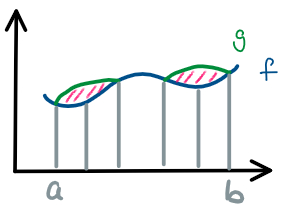
\includegraphics[scale=0.5]{Skizzen/plot_integral_zwei_fkt}
		\end{center}
		\caption{Flächeninhalt zweier Funktionen}
		\label{plot_flaeche_zweier_fkt}
	\end{figure}
	
	\item für $c \in [a,b]$ soll gelten (Abbildung~\ref{fig_integral_aufteilen})
	\begin{align*}
		\int_a^b f \dd{x} = \int_a^c f \dd{x} + \int_c^b f\dd{x}
	\end{align*}
	Vorgehen: Man unterteile $[a,b]$ in \enquote{viele} Teilintervalle, auf denen 
	$f$ nahezu konstant ist.
	\begin{figure}[ht]
\centering
	\begin{tikzpicture}
		\draw[very thin, gray, step = 0.5] (-0.9,-0.9) grid (4.9,2.9);
		\draw[->,thick, black](-1,0) -- (5,0) node[right]{x};
		\draw[->,thick, black](0,-1) -- (0,3) node[above]{y};
		\draw[blue,domain = 0.0:3.14, samples=1000]   
			plot (\x,{(\x * \x)*sin(\x r)*0.5+0.5});
       	\draw[green,thick](0.0,0)--(0.0,2.5)node[right]{a};
       	\draw[red,thick](3.14,0) -- (3.14,2.5) node[above]{b};
       	\draw[orange,thick](1.5,0) -- (1.5, 1.62) node[above]{c};
	\end{tikzpicture}
	\caption{Integral aufteilen}
	\label{fig_integral_aufteilen}
\end{figure}
\end{itemize} 

\begin{Definition}{
	Sei $ I \subseteq \mathbb{R}$ ein Intervall. Eine \underline{Partition}\todo{das geht besser auch mit Stichwortverzeichnis. Baue ich später ein.} $P$ 
	(Abbildung~\ref{fig_int_partition}) von 
	$[a,b]$ ist eine endliche Menge von Punkten $a = x_0 \leq x_1 \leq \hdots
	\leq x_n = b$.\\
	Wir schreiben $\Delta x_i = x_i - x_{i-1}$
	\begin{figure}[ht]
       \tikzsetnextfilename{plot_integral_partition}
       \begin{center}
              \begin{tikzpicture}
       		\draw[dotted, very thin, gray, step = 0.5] (-0.9,-0.9) grid (4.9,2.9);
       		\draw[->,thick, black](-1,0) -- (5,0) node[right]{x};
       		\draw[->,thick, black](0,-1) -- (0,3) node[above]{y};
       		\draw[blue,domain = 0.0:3.14, samples=1000]   
       			plot (\x,{(\x * \x)*sin(\x r)*0.5+0.5});
              	\draw[green,thick](0.0,0)--(0.0,2.5)node[right]{a};
              	\draw[red,thick](3.14,0) -- (3.14,2.5) node[above]{b};
              	\draw[black,thick](0.25,0) -- (0.25, 0.5)node[above]{$x_1$};
              	\draw[black,thick](0.5,0) -- (0.5, 0.55);
              	\draw[black,thick](1,0) -- (1, 0.92);
              	\draw[black,thick](1.25,0) -- (1.25, 1.24);
              	\draw[black,thick](1.5,0) -- (1.5, 1.62);
              	\draw[black, thick](2,0) -- (2, 2.31) node[above]{$x_i$};
              	\draw[black,thick](2.5,0) -- (2.5, 2.37);
              	\node at (4,1.5){$\int_a^b f$};
       	\end{tikzpicture}
       \end{center}
	\caption{Partition}
	\label{fig_int_partition}
\end{figure}
}\end{Definition}

\begin{Definition}{ \label{def_riemann-integrierbar}
	Sei $f : [a,b] \rightarrow \mathbb{R}$ beschränkt und $P = \{x_0, \hdots, x_n\}$ 
	eine Partition von $[a,b]$.\\
	Wir schreiben: 
	\begin{align*}
		M_i(P) := \sup_{x \in [x_{i-1}, x_i]} f(x) \\
		m_i(p) := \inf_{x \in [x_{i-1}, x_i]} f(x)
	\end{align*}
	Weiter definieren wir: 
	\begin{align*}
		S(P,f) := & \sum_{i=1}^n M_i \cdot \Delta x_i \\
		s(P,f) := & \sum_{i=1}^n m_i \cdot \Delta x_i
	\end{align*}
	Wir setzen:
	\begin{align*}
		\overline{\int_a^b} f \dd{x} = \inf S(P,f) \\
		\underline{\int_a^b} f \dd{x} = \sup s(P,f)
	\end{align*}
	wobei Infimum und Supremum über alle Partitionen von $[a,b]$ genommen werden. 
	Wir nennen 
	\begin{align*}
		& \overline{\int_a^b} f \dd{x} \text{ das \underline{obere} und} \\
		& \underline{\int_a^b} f \dd{x} \text{ das \underline{untere}}
	\end{align*}
	\underline{Riemannintegral} von $f$ über $[a,b]$ \\
	Gilt 
	\begin{align*}
		\int_a^{\overline{b}} f \dd{x} = \int_{\underline{a}}^b f \dd{x}
	\end{align*}
	sagen wir $f$ ist \underline{Riemann-integrierbar} (\underline{integrierbar}) 
	und nennen 
	\begin{align*}
		\int_a^b f(x) \dd{x} := \underline{\int_a^b} f \dd{x} = 
		\overline{\int_a^b} f \dd{x}
	\end{align*}
	das \underline{Riemannintegral} von $f$ über $[a,b]$.\\
	Die Menge der Riemanintegrierbaren Funktionen auf $[a,b]$ bezeichnen wir 
	mit $\mathcal{R}$ beziehungsweise $\mathcal{R}_{[a,b]}$.\\
	\begin{figure}[ht]
\centering
	\begin{tikzpicture}
		\draw[very thin, gray, step = 0.5] (-1.9,-0.9) grid (1.9,3.4);
		\fill[yellow](-1.5,0) rectangle (-0.75,3.25);
		\fill[orange](-0.75,0) rectangle (0,1.56);
		\fill[yellow](0,0) rectangle (0.75, 1.56);
		\fill[orange](0.75,0) rectangle (1.5,3.25);
		\draw[->,thick, black](-2,0) -- (2,0) node[right]{x};
		\draw[->,thick, black](0,-1) -- (0,3.5) node[above]{y};
		\draw[blue, domain = -1.5 :1.5]  
			plot(\x, \x * \x + 1);
	\end{tikzpicture}
	\caption{oberes Riemann-Integral}
	\label{fig_int_riemann}
\end{figure}
	\textbf{Bemerkungen}
	\begin{itemize}
		\item Da $f$ beschränkt ist, gibt es $m \leq M$ in $\mathbb{R}$ mit:
		\begin{align*}
			m \leq f(x) \leq M \text{ }(x \in [a,b])
		\end{align*}
		Damit gilt für jede jede Partition $P$: 
		\begin{align*}
			m \cdot (b-a) \leq s(P,f) \leq S(P,f) \leq M \cdot (b-a)
		\end{align*}
		Ergo: $\overline{\int_a^b} f \dd{x} , \underline{\int_a^b} f \dd{x}$ 
		sind wohldefiniert.
		\item im gesamten Kapitel~\ref{kap_riemann_integral}
		werden wir Funktionen stets als 
		beschränkt annehmen
	\end{itemize}
	
}\end{Definition}

\begin{Definition}{
	Seien $P_1, P_2$ zwei Partitionen eines Intervalls. Dann heißt $P_1$ 
	\underline{Verfeinerung} von $P_2$, wenn gilt: $P_2 \subseteq P_1$ \\
	Weiterhin nennen wir $P_1 \cup P_2$ die \underline{gemeinsame} Verfeinerung 
	von $P_1$ und $P_2$
}\end{Definition}

\begin{Satz}{\label{kap09_satz16}
	Ist $P'$ eine Verfeinerung der Partition $P$ von $[a,b]$, dann gilt:
	\begin{align*}
		S (P,f) \geq & S (P',f) \\
		s(P,f) \leq & s(P',f)
	\end{align*}
	(wobei $f$ wie in Definition~\ref{def_riemann-integrierbar}
	sei) \\
	\textbf{Beweis:} Wir zeigen nur die obere Ungleichung, die andere folgt analog. 
	Wir nehmen zunächst an, dass $P'$ sich von $P$ in nur einem Element $x'$ 
	unterscheidet. Das heißt: $P' = P \cup \{x'\}$ \\
	Dann gibt es ein $i \in \mathbb{N}$ mit $x' \in [x_{i-1}, x_i]$ \newline
	(wobei $P = \{x_0, x_1, \hdots, x_{i-1}, x_i, \hdots, x_n \}$ sei).\\
	Wir definieren:
	\begin{align*}
		W_1 := & \sup_{[x_{i-1}, x']} f(x) \\
		W_2 := & sup_{[x', x_i]} f(x)
	\end{align*}
	Dann gilt: 
	\begin{align*}
		S(P,f) - S(P',f) = &M_i \Delta x_i - W_1\cdot (x' - x_{i-1}) - 
		W_2\cdot (x_i - x') \\
		= & (M_i -W_1) \cdot (x' - x_{i-1}) 
		+ (M_i - W_2)\cdot(x_i - x') \geq 0
	\end{align*}
	 Enthält von $P'$ $k$ Punkte, die nicht in $P$ enthalten sind, so führen wir 
	 obiges Verfahren insgesamt $k$-mal durch. 
	
}\end{Satz}

\begin{Satz}{\label{kap09_satz17}
	Sei $f: [a,b] \rightarrow \mathbb{R}$ beschränkt. Dann gilt:
	\begin{align*}
		\obint a b f \geq \unint{a}{b} f
	\end{align*}
	\textbf{Beweis:} Seien $P_1, P_2$ zwei Partitionierungen von $[a,b]$ und 
	$P'$ die gemeinsame Verfeinerung. Dann gilt:
	\begin{align*}
		s(P_1,f) \leq s(P',f) \leq S(P',f) \leq S(P_2, f) 
	\end{align*}
	Mit anderen Worten:
	\begin{align*}
		s(P_1, f) \leq S(P_2, f)
	\end{align*}
	für alle Partitionierungen $P_1, P_2$. \\
	Sprich: $S(P_2,f)$ ist stets obere Schranke von $s(P,f)$ für alle Partitionen 
	$P$ von $[a,b]$. Ergo:
	\begin{align*}
		\sup s(P,f) \leq S (P_2, f)
	\end{align*}
	Damit ist also $\sup s(P,f)$ untere Schranke von $S(P,f)$ ($P$ beliebige 
	Partition). \\
	Ergo: $\sup s(P,f) \leq \inf S (P,f)$  \\
	Wir haben also gezeigt:
	\begin{align*}
		\int_{\underline{a}}^b f \dd{x} = \sup s(P,f) \leq 
		\inf S(P,f) = \inf \obint ab f 
	\end{align*}
}\end{Satz}
%!TEX root = ../gesamt.tex

\begin{Satz}{\label{kap_10_satz18}
	Sei $f: [a,b] \rightarrow \mathbb{R}$ beschränkt. Dann ist 
	$f \in \mathcal{R}_{[a,b]}$ genau dann, wenn für jedes $\epsilon > 0$ eine 
	Partition $P_{\epsilon}$ existiert mit:
	\begin{align*}
		S(P_2,f) - s(P_2,f) < \epsilon
	\end{align*}
}\end{Satz}

\begin{proof}
	 Per Definition gilt 
	\begin{align*}
		s(P_{\epsilon},f) \leq \underline{\int_{a}^b} f \dd{x}
		\overset{Satz~\ref{kap09_satz17}}{\le} \overline{\int_a^b} f \dd{x} 
		\leq S(P_{\epsilon},f) 		
	\end{align*}

	Damit erhalten wir:
	\begin{align*}
		\overline{\int_a^b} f \dd{x} - 
		\underline{\int_{a}^b} f \dd{x} \leq S(P_{\epsilon},f) 
		- s(P_{\epsilon},f) < \epsilon
	\end{align*}
	Das heißt, da $\epsilon$ beliebig, dass:
	\begin{align*}
		\underline{\int_{a}^b} \dd{x} = \overline{\int_a^b} f \dd{x}
	\end{align*}
	Ergo: $f \in \mathcal{R}_{[a,b]}$ \\
	Per Definition gibt es für alle $\epsilon > 0$ ein $P_{\epsilon}'$ mit:
	\begin{align}
		\label{gleichung_1_1505}
		\underline{\int_{a}^b} f \dd{x} - s(P_{\epsilon}',f) < \frac{\epsilon}{2} 
	\end{align}
	Analog existiert ein $P_{\epsilon}''$ mit 
	\begin{align}
		\label{gleichung_2_1505}
		S(P_{\epsilon}'',f) - \overline{\int_a^{b}} f \dd{x}) < \frac{\epsilon}{2}
	\end{align}
	Wir setzten $P_{\epsilon}$ gleich der gemeinsamen Vereinigung von 
	$P_{\epsilon}'$ und $P_{\epsilon}''$. Man beachte: Wegen Satz~\ref{kap09_satz16} 
	gelten Gleichung~\ref{gleichung_1_1505} und Gleichung~\ref{gleichung_2_1505},
	wenn wir $P_{\epsilon}'$, beziehungsweise $P_{\epsilon}''$, durch $P_{\epsilon}$
	ersetzen. Da $f \in \mathcal{R}_{[a,b]}$ gilt außerdem:
	\begin{align*}
		\underline{\int_{a}^b} f \dd{x} = \overline{\int_a^{b}} f\dd{x}
	\end{align*}	 
	Addition von Gleichung~\ref{gleichung_1_1505} und Gleichung~
	\ref{gleichung_2_1505} liefert:
	\begin{align*}
	S(P_{\epsilon},f) - s(P_{\epsilon},f) < \epsilon
	\end{align*}
\end{proof}

\begin{Satz}{\label{kap10_satz19}
	Sei $f:[a,b] \rightarrow \mathbb{R}$ beschränkt und $P_{\epsilon} = 
	\{x_0, \hdots, x_n\}$ eine Partition von $[a,b]$ mit $S(P_{\epsilon},f) -
	s(P_{\epsilon},f) < \epsilon$ für ein $\epsilon > 0$.
	\begin{enumerate}
		\item Ist $P$ eine Verfeinerung von $P_{\epsilon}$, so gilt 
		$S(P,f) - s(P,f) < \epsilon$
		\item Sind $s_i, t_i$ beliebige Punkte in $[x_{i-1},x_i]$, so gilt:
		\begin{align*}
			\sum_{i=1}^n \left\vert f(s_i) - f(t_i) \right\vert \cdot 
			\Delta x_i < \epsilon
		\end{align*}
		\item Ist $f \in \mathcal{R}_{[a,b]}$ und $t_i \in [x_{i-1},x_i]$, so 
		gilt 
		\begin{align*}
			\left\vert \sum_{i=1}^n f(t_i) \cdot \Delta x_i - \int_a^b f \dd{x} 
			\right\vert < \epsilon
		\end{align*}
	\end{enumerate}	
}\end{Satz}

\begin{proof}
	\begin{enumerate}
		\item[ ]
		\item Das folgt aus Satz~\ref{kap09_satz16}
		\item
		 \begin{align*}
			\sum_{i = 1}^n \left\vert f(s_i) - f(t_i) \right\vert	\cdot 
			\Delta x_i \leq \sum_{i=1}^n (M_i-m_i)\cdot \Delta x_i
			= S(P_{\epsilon},f) - s(P_{\epsilon},f) < \epsilon
		 \end{align*}
		 \item Da $t_i \in [x_{i-1},x_i]$, gilt $m_i \leq f(t_i) \leq M_i$ \\
		 	Damit folgt die Aussage aus
			 \begin{align*}
			 	s(P_{\epsilon},f ) \leq  
			 	\sum_{i = 1}^n m_i \cdot \Delta x_i \leq \sum_{i=1}^n f(t_i) \cdot \Delta 
			 	x_i \leq \sum_{i=1}^n M_i \cdot \Delta x_i = S(P_{\epsilon},f)
			 \end{align*}
			 und $s(P_{\epsilon},f) \leq \int_a^b f \dd{x} \leq S(P_{\epsilon},f)$
	\end{enumerate}
\end{proof}
	Wir wollen im Folgenden wichtige Vertreter Riemann-integrierbarer 
	Funktionen kennenlernen.

\begin{Satz}{\label{kap10_satz20}
	Ist $f: [a,b] \rightarrow \mathbb{R}$ stetig, so ist 
	$ f \in \mathcal{R}_{[a,b]}$.
}\end{Satz}

\begin{proof}
	Da stetige Funktionen auf abgeschlossenen Intervallen 
	beschränkt sind, ist $f$ offensichtlich beschränkt. Weiterhin ist $f$ als stetige 
	Funktion auf dem abgeschlossenen Intervall $[a,b]$ gleichmäßig stetig. \\
	Sei $\epsilon > 0 $ gegeben. Wegen der gleichmäßigen Stetigkeit von $f$ 
	existiert ein $\delta > 0$, so dass folgende Implikation gilt:
	\begin{align*}
		\vert x - y \vert < \delta \Rightarrow \vert f(x) -f(y) \vert < \epsilon
	\end{align*}
	Wir wählen eine Partition $P_{\epsilon} = \{ x_0, \hdots, x_n \}$, so dass 
	$\Delta x_i < \delta$. Dann gilt:
	\begin{align*}
		M_i - m_i < & \epsilon \text{ und daher} \\
		S(P_{\epsilon},f) - s(P_{\epsilon},f) = & \sum_{i = 1}^n (M_i -m_i)\Delta x_i 
		\leq \epsilon \cdot \sum_{i = 1}^n \Delta x_i = \epsilon \cdot (b-a)
	\end{align*}
	Da $\epsilon > 0$ beliebig, folgt die Aussage mit Satz~\ref{kap_10_satz18}.
\end{proof}

\begin{Satz}{
		Ist $f: [a,b] \rightarrow \mathbb{R}$ monoton, so ist 
		$f \in \mathcal{R}_{[a,b]}$ 
}\end{Satz}

\begin{proof}
	 Da $f$ monoton ist, gilt für alle $x \in [a,b]: f(a) \leq f(x) 
	\leq f(b)$. \\
	Das heißt $f$ ist beschränkt. Zu $n \in \mathbb{N}$ wählen wir eine 
	Partition \linebreak $P_n = \{x_0, \hdots, x_k\}$ mit $\Delta x_i < \frac{1}{n}$.
	\begin{figure}
	\begin{center}
	\tikzsetnextfilename{monotone_fkt_riemann_intbar}
		\begin{tikzpicture}
			\draw[very thin, gray, step = 0.5] (0,-0.9) grid (3.4,2.4);
			
			\draw[->, thick, black](0,-0.5) -- (3.5,-0.5) node[right]{x};
			\draw[->, thick, black](0.5, -1) -- (0.5, 2.5) node[above]{y};
			\draw[blue, domain = 1 :1.5, samples = 1000]  
				plot(\x, {\x * \x * sin(\x r) - \x });
			
			\draw[blue, domain = 2 :3, samples = 1000]  
				plot(\x, {\x * \x * sin(0.5*\x r) - \x*\x + 2});	
			
			\draw[fill=black](1,-0.16)circle(1pt);
			\draw[fill = black](1.3,0.33) circle(1pt);
			\draw[fill = black] (1.5, 0.74) circle(1pt);
			\draw[thick, black](1,-0.5) -- (1, -0.16);
			\draw[thick, black](1.3,-0.5) --(1.3, 0.33);
			\draw[thick, black](1.5,-0.5) --(1.5, 0.74);
			
			\draw[fill = black](2.1,1.42) circle (1pt);
			\draw[fill = black](2.9,1.94) circle(1pt);
			\draw[thick, black](2.1, -0.5) -- (2.1, 1.42);
			\draw[thick, black](2.9, -0.5) -- (2.9, 1.94);
		
		\end{tikzpicture}
	\end{center}
	\caption{Monotone Funktion}
	\label{fig:Monotone_Funktion_Riemannint}
\end{figure}
	Dann gilt:
	\begin{align*}
		S(P_n, f) - s(P_n,f) = & \sum_{i=1}^n (M_i - m_i)\Delta x_i
	\end{align*}
	Ohne Einschränkung sei $f$ monoton wachsend (der andere Fall läuft analog).
	Dann gilt:
	\begin{align*}
		M_i = & f(x_i) \text{ und} \\
		m_i = & f(x_{i-1})
	\end{align*} und daher:
	\begin{align*}
		S(P_n, f) - s(P_n,f) = & \sum_{i=1}^n (f(x_i) -f(x_{i-1}))\cdot \Delta x_i 
		\\ \leq & \frac{1}{	n}\sum_{i=1}^n f(x_i) -f(x_{i-1}) = 
		\frac{1}{n} (f(b) -f(a)) 
	\end{align*}
	Sei $\epsilon > 0$ gegeben. Wähle $n_{\epsilon}$ so dass gilt:
	\begin{align*}
		\frac{1}{n_{\epsilon}}(f(b) -f(a)) < \epsilon
	\end{align*}
	Dann gilt mit $P_{\epsilon} := P_{n_{\epsilon}}$ die Aussage nach Satz~\ref{kap_10_satz18}
\end{proof}

\begin{Satz}{\label{kap10_satz21}
	Sei $f: [a,b] \rightarrow \mathbb{R}$ beschränkt mit endlich vielen 
	Unstetigkeitsstellen %(Abbildung~\ref{plot_fkt_unstetigketsstellen}. 
	Dann gilt $f \in \mathcal{R}_{[a,b]}$.\\
	\begin{figure}[ht]
		\begin{center}
			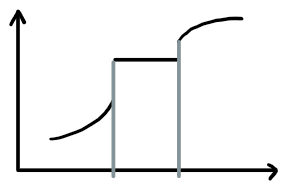
\includegraphics[scale=0.5]{Skizzen/plot_fkt_unstetigkeitsstellen}
		\end{center}
		\caption{Funktion mit endlich vielen Unstetigkeitsstellen}
		\label{plot_fkt_unstetigketsstellen}
	\end{figure}
}\end{Satz}

\begin{proof}
	 Sei $\epsilon > 0$ gegeben und $E = \{P_1, \hdots, P_n\}$
	die Menge der Unstetigkeitsstellen von $f$. Wir nehmen der Einfachheit halber 
	an, dass $\{a,b\} \cap E = \emptyset$ (der andere Fall läuft analog).
	Sei
	\begin{align*}
		 M:= \sup_{x \in [a,b]} \vert f(x) \vert
	\end{align*}
	 Wir wählen $u_j, v_j \in [a,b]$, 
	$j = (1, \hdots, n)$, so dass
	\begin{align*}
		P_s \in [u_j, v_j] \text{ und} \\
		2M (u_j - v_j) < \frac{\epsilon}{2n}
	\end{align*}		
	 Sei 
	 \begin{align*}
		I_1^{\epsilon} = & [a, u_1], \\
		 I_l^{\epsilon} = & [v_{l-1}, u_l] \text{ }  (l = 2, \hdots, n) \\
		 I_n^{\epsilon} = & [v_n, b]
	 \end{align*}
	Per Voraussetzung ist $f_{\vert I_j^{\epsilon}} (j = 1,\hdots, n+1)$ stetig. \\
	Daher existiert nach Satz~\ref{kap10_satz20}
	eine Partition $P_j^{\epsilon}$, so dass:
	\begin{align*}
		S(P_j^{\epsilon}, f_{I_j{\epsilon}}) - s(P_j^{\epsilon}, f_{I_j^{\epsilon}}) 
		 < \frac{\epsilon}{2(n+1)}
	\end{align*}
	Wir setzen $P^{\epsilon} = \cup_{l = 1}^n P_l^{\epsilon}
	 \cup U_{l=1}^n\{u_l,v_l\}$.\\
	 Dann gilt:
	 \begin{align*}
	 	S(P^{\epsilon},f) - s(P^{\epsilon},f) 
	 	= & \sum_{l=1}^{n+1} S(P_l^{\epsilon},f_{|I_l^{\epsilon}}) - 
	 		s(P_l^{\epsilon},f_{|I_l^{\epsilon}})  \\
	 		& + \sum_{l = 1}^n \left( \sup_{x \in [u_l, v_l]} 
	 		f(x) - \inf_{x \in [u_l, v_l]} f(x) (v_l - u_l)\right) \\
	 		\leq & \sum_{l=1}^{n+1} \frac{\epsilon}{2(n+1)} + \sum_{l=1}^n
	 			2M \cdot(v_l-u_l) \leq \frac{\epsilon}{2} + \frac{\epsilon}{2} 
	 			= \epsilon
	 \end{align*}	 
\end{proof}

\begin{Definition}{
	Eine Funktion $f: [a,b] \rightarrow \mathbb{R}$ heißt \emph{Treppenfunktion}
	 (Abbildung~\ref{plot_treppenfkt}), 
	wenn es 
	eine Partition $Z = \{ y_0, \hdots, y_m \}$ von $[a,b]$ gibt und für alle 
	$i \in \{0, \hdots, m\}$ für $c_i \in \mathbb{R}$ gibt, so dass:
	\begin{align*}
		f(x) = c_i \text{ } ( x\in (y_{i-1},y_i))
	\end{align*}
	gilt.
	\begin{figure}
		\begin{center}
			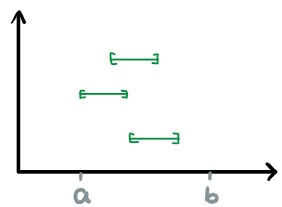
\includegraphics[scale=0.5]{Skizzen/plot_treppenfkt}
		\end{center}
		\caption{Treppenfunktion}
		\label{plot_treppenfkt}
	\end{figure}
	Nach Satz~\ref{kap10_satz21}
	ist jede Treppenfunktion Riemann-integrierbar. \\
	Zur Berechnung des Intervalls bedienen wir uns der Notation von Satz 10 
	\todo{falsche Referenz -> hardgecodet; sollte Satz 3.7 sein}
	%\ref{kap10_satz21}
	und verwenden Satz~\ref{kap10_satz19}c.\\
	Zur Vereinfachung nehmen wir wieder an, dass $f$ in $a$ und $b$ stetig ist. 
	Das heißt die Menge der Unstetigkeitsstellen ist gegeben durch 
	$E = \{y_1, \hdots, y_{m-1}\}$. \\
	Für $x \in I_l^{\epsilon}$ gilt dann $f(x) = c_l$ für alle $ l = 1, \hdots, m$.
	Dann gilt nach Satz~\ref{kap10_satz19}c:
	\begin{align*}
		\left\vert \int_a^b f \dd{x} - \sum_{i=1}^{m+1} c_i \cdot \vert 
		I_l^{\epsilon}\vert + \sum_{i =1}^{m-1} f(y_i)\cdot (v_i -u_i) \right\vert
		< \epsilon
	\end{align*}
	Für $ \lim\limits_{\epsilon \rightarrow 0}{}$ gilt:
	$$\begin{cases} 
		|I_1^\epsilon| \rightarrow y_{1}-a & \\
		\vert I_l^\epsilon \vert \rightarrow y_l - y_{l-1} & ( l = 2,...,m) \\
		\vert I_{m+1}^{\epsilon} \vert \rightarrow b - y_m &
	\end{cases}$$
	Das heißt
	\begin{align}
		\label{gleichung_3_1705}
		\sum_{i=1}^{m+1}c_i \abs{I^{\epsilon}_l} \rightarrow c_1(y_1 -a) + 
		\sum_{i=2}^m c_i \cdot (y_i -y_{i-1}) + c_m(b-y_m)
	\end{align}
	Außerdem gilt $v_i-u_j \overset{\epsilon \rightarrow 0}{\rightarrow} 0$
	gilt $\int_a^b f\dd{x} = Gleichung~\ref{gleichung_3_1705}$
	
}\end{Definition}

\begin{Korollar}{
	Ist $f:[a,b] \rightarrow \mathbb{R}$ stetig, beziehungsweise monoton, beziehungsweise 
	besitzt $f$ höchstens endlich viele Unstetigkeitsstellen und ist beschränkt, so ist 
	$f \in \mathcal{R}_{[a,b]}$.
}\end{Korollar}

\begin{Bemerkung}{
	Mit Hilfe des Lebesguesches Integrabilitätskriterium kann man 
	sogar zeigen, dass beschränkte Funktionen mit abzählbar vielen Unstetigkeitsstellen 
	Riemann-integrierbar sind.
}\end{Bemerkung}

\begin{Beispiel}{
	\begin{align*}
		\int_0^a x \dd{x}
	\end{align*}
	Da $id :[0,a] \rightarrow \mathbb{R}$ stetig ist, existiert das Integral. \\
	Sei $P_n =\{ 0, \frac{a}{n}, \frac{2a}{n}, \hdots, \frac{(n-1)a}{n}, a\}$ 
	eine Partition von $[a,b]$. \\
	Es gilt: 
	\begin{align*}
		S(P_n, x) = & \sum_{i =1} ^n \frac{a_i}{n} \cdot \frac{a}{n} \\
		= & \frac{a^2}{n^2} \sum_{i = 1}^n i \\
		= & \frac{a^2}{n^2} \frac{n(n+1)}{2} \\ 
		= & \frac{a^2}{2} \cdot \left( 1 + \frac{1}{n} \right)
	\end{align*}
	\begin{align*}
		s(P_n, x) = & \sum_{i = 0}^n \frac{a_i}{n} \cdot \frac{a}{n}  \\
		= & \frac{a^2}{n^2} \cdot \frac{(n-1)n}{2} \\
		= & \frac{a^2}{2}\left( 1 - \frac{1}{n} \right)
	\end{align*}
	Da $id$ integrierbar ist, gilt:
	\begin{align*}
		\int_0^a x \dd{x} \in \left[ s(P_n,x), S(P_n, x)\right] = 
		\left[\frac{a^2}{2}- \frac{1}{n}, \frac{a^2}{2}+\frac{1}{n}\right]
		n \in \mathbb{N}
	\end{align*}
	Das heißt:
	\begin{align*}
		\int_0^a x \dd{x} \cap_{n \in \mathbb{N}} \left[\frac{a^2}{2}- \frac{1}{n}, 
		\frac{a^2}{2}+\frac{1}{n}\right]
	\end{align*}
	Also: $\int_0^a x \dd{x} = \frac{a^2}{2}$
}\end{Beispiel}

\begin{Beispiel}{
	Sei $D:[0,1] \rightarrow \mathbb{R}$ die \emph{Dirichlet-Funktion}, d.h
	\begin{align*}
		D(x) = \begin{cases}
			1 & \textit{falls } x \in \mathbb{Q} \\
			0 & sonst
		\end{cases}
	\end{align*}
	Daher gilt für jede Partition $P = \{x_0, \hdots, x_n\}$, dass 
	\begin{align*}
		M_i = & \sup_{x \in [x_{i-1}-x_i]} f(x) = 1 \text{ und}\\
		m_i = & \inf_{x \in [x_{i-1}-x_i]} f(x) = 0
	\end{align*}
	Damit gilt:
	\begin{align*}
		S(P,f) - s(P,f) = \sum_{i = 1}^n (M_i - m_i) \cdot \Delta x_i 
		= \sum_{i = 1}^n \Delta x_i = 1
	\end{align*}
	Ergo: $D$ ist nicht Riemann-integrierbar
}\end{Beispiel}

\begin{Satz}{\label{vl_11_satz23}
	Sei $f \in \mathcal{R}_{[a,b]}$ und $m \leq f(x) \leq M$ $ (x \in [a,b])$.
	Sei ferner  \linebreak $\Phi : [m, M] \rightarrow \mathbb{R}$ stetig. 
	Dann ist $\Phi \circ f \in \mathcal{R}_{[a,b]}$ \\
	\textbf{Beweis:} Sei $\epsilon > 0$ gegeben. Da $\Phi$ auf dem abgeschlossenen Intervall 
	$[m,M]$ stetig ist, existiert ein $\delta > 0$ 
	(Ohne Eisnchränkung sei $\delta < \epsilon$) mit :
	\begin{align*}
		\vert s - t\vert < \delta \Rightarrow \vert f(x) - f(t) \vert < \epsilon
	\end{align*}
	Da $f$ integrierbar ist, gibt es eine Partition $P = \{x_0, \hdots, x_n\}$
	mit 
	\begin{align*}
		S(P,f) - s(P,f) < \delta^2
	\end{align*}		
	Wie üblich bezeichnen wir 
	\begin{align*}
		M_i = & \sup_{x \in [x_{i-1}-x_i]} f(x) \text{ und } \\
		m_i = & \inf_{x \in [x_{i-1}-x_i]} f(x) \text{ und weiterhin} \\
		M_i^+ = & \sup_{x \in [x_{i-1}-x_i]} \Phi \circ f \text{ sowie } \\
		m_i^* = & \inf_{x \in [x_{i-1}-x_i]} \Phi \circ f(x)
	\end{align*}		
	Seien
	\begin{align*}
		A = & \{i = 1, \hdots, n \vert M_i -m < \delta \} \\
		B = & \{ i = 1, \hdots, n\} \setminus A
	\end{align*}
	Aufgrund der Wahl von $\delta$ gilt für alle $ i \in A: M_I^+ - m_i^* < \epsilon$
	Weiter gilt: 
	\begin{align*}
		\delta \cdot \sum_{i \in B} \Delta x_i = \sum_{i \in B} \delta \cdot \Delta x_i 
		\leq  \sum_{i \in B} (M_i - m_i) \Delta x_i \leq \delta^2
	\end{align*}
	Ergo: $\sum_{i \in B} \Delta x_i \leq \delta$. \\
	Damit gilt:
	\begin{align*}
		S(P, \Phi \circ f) - s(P, \Phi \circ f) = 
		& \sum_{i = 1}^n (M_i^+ - m_i^*) \cdot\Delta x_i  \\
		= & \sum_{i \in A} (M_i^+ - m_i^* ) \cdot \Delta x_i + 
			\sum_{i \in B} (M_i^+ -m_i) \Delta x_i \\
		\leq & \epsilon \sum_{i \in A}\Delta x_i + 2 \sup_{x \in [m,M]} \abs{
			\Phi \circ f} \cdot \sum_{i \in B} \Delta x_i \\
		\leq & \epsilon \left(|b-a| + 2\sup_{x \in [m,M]} \abs{\Phi \circ f(x)}\right)
	\end{align*}
	Da $\epsilon > 0$ beliebig, folgt die Behauptung mit~\ref{kap_10_satz18}.
}\end{Satz}

\begin{Satz}{\label{vl_11_satz24}%12
	Seien $f_1, f_2,f \in \mathcal{R}_{[a,b]}$ Dann gilt:
	\begin{enumerate}
		\item 
		\begin{align*}
			\int_a^b f_1 +f_2 \dd{x} = \int_a^b f_1\dd{x} + \int_a^b f_2 \dd{x}
		\end{align*}
		und für $c \in \mathbb{R}$ gilt:
		\begin{align*}
			\int_a^b c f\dd{x} = c \int_a^b f\dd{x}
		\end{align*}
		\item Insbesondere gilt also 
		\begin{align*}
			f_1 + f_2 \in \mathcal{R}_{[a,b]} \text{und} \\
			c f \in \mathcal{R}_{[a,b]}
		\end{align*}
		\item Gilt $f_1(x) \leq f_2(x) \text{ } ( x \in [a,b])$ so folgt
		\begin{align*}			
			\int_a^b f_1 \dd{x} \leq \int_a^b f_2 \dd{x}
		\end{align*}
		\item Ist $c \in (a,b)$, und $f \in \mathcal{R}_{[a,b]}$ so gilt
		\begin{align*}
			\int_a^b f\dd{x} = \int_a^c f\dd{x} + \int_c^b f \dd{x}
		\end{align*}
		\item Gilt $M \geq f(x)$ $(x \in [a,b])$ so gilt 
		\begin{align*}
			M \cdot (b-a) \geq \int_a^b f \dd{x}
		\end{align*}
	\end{enumerate}
	\textbf{Beweis:}
	\begin{enumerate}
		\item Da $f_i \in \mathcal{R}_{[a,b]} (i = 1, 2)$ gibt es Partitionen 
		$P_i$ von $[a,b]$ mit 
		\begin{align*}
			S(P_i,f) - s(P_i,f) \leq \epsilon \text{ für ein festes } \epsilon > 0
		\end{align*}
		Dann gilt für die gemeinsame Verfeinerung $P = P_1 \cup P_2 = \{x_0, \hdots
		x_n\}$ nach Satz~\ref{kap09_satz16}
		, dass 
		\begin{align*}
			S(P,f_i) - s(P, f_i) \leq \epsilon \text{ }(i = 1,2)
		\end{align*}		 
		\item Es gilt 
		\begin{align*}
			\sup_{x \in [x_{i-1}-x_i]} f_1(x) +f_2(x) \leq & 
			\sup_{x \in [x_{i-1}-x_i]} f_1(x) + \sup_{x \in [x_{i-1}-x_i]} f_2(x)
		\end{align*}				
		Analog gilt: 
		\begin{align*}
			\inf_{x \in [x_{i-1}-x_i]} f_1(x) + f_2(x) \geq & 
			\inf_{x \in [x_{i-1}-x_i]} f_1(x) + \inf_{x \in [x_{i-1}-x_i]} f_2(x)
		\end{align*}				
		Damit folgt:
		\begin{align*}
			s(P,f_1) + s(P,f_2) \leq s(P,f_1 +f_2) \leq S(P,f_1 + f_2) 
			\leq S(P,f_1) + S(P,f_2)
		\end{align*}
		Also gilt:
		\begin{align*}
			S(P, f_1 + f_2) - s(P, f_1 +f_2) & \\
			\leq &  S(P, f_1) - s(P,f_1) + S(P,f_2) 
			-s(P,f_2) \leq 2 \epsilon
		\end{align*}
		Da $\epsilon >0 $ beliebig gewählt war, gilt $f_1 + f_2 \in 
		\mathcal{R}_{[a,b]}$ nach Satz~\ref{kap_10_satz18}. \\
		Weiter gilt: 
		\begin{align*}
			s(P, f_1 +f_2), S(P, f_1 + f_2) \in &
			[s(P,f_1) - s(P,f_2), S(P,f_1) + S(P,f_2)] \\
			\subseteq 
			& \left[ \int_a^b f_1 \dd{x} + \int_a^b f_2\dd{x} + 2\epsilon \right]
		\end{align*}
		Da $\epsilon > 0$ beliebig gewählt wurde, gilt:
		\begin{align*}
			\int_a^b f_1 + f_2 \dd{x}  = \int_a^b f_1\dd{x} + \int_a^b f_2 \dd{x}
		\end{align*}
		Die Aussage bezüglich  $c \cdot f$ zeigt man analog.
		\item Sei $f_2(x) \geq f_1(x)$ $(x \in [a,b])$. Dann gilt
		\begin{align*}		
			f_2(x) - f_1(x) \geq & 0 \text{ und daher} \\
			s(P, f_2 -f_1) \geq & 0
		\end{align*} 
		 für jede Partition $P$ von $[a,b]$ 
		Wegen 1 ist $f_2 -f_1 \in \mathcal{R}_{[a,b]}$ und es gilt:
		\begin{align*}
			\int_a^b f_2 \dd{x} = \int_a^b f_1 \dd{x} + \int_a^bf_2-f_1 \dd{x} 
			\geq \int_a^b f_1 \dd{x}
	\end{align*}		 
	\item Für 3. betrachtet man zu beliebiger Partition $P$ von $[a,b]$ die Partition \linebreak
	$P' = \{c\} \cup P$
	\item Folgt aus 2. mit $f_1 = f$ und $f_2 = M$ soweit 
	\begin{align*}
		\int_a^b M \dd{x} = M \cdot (b-a)
	\end{align*}		
	\end{enumerate}
}\end{Satz}

\begin{Bemerkung}{
	\begin{itemize}
	 	\item[ ]
		\item Eigenschaft 1 sagt, dass $\mathcal{R}_{[a,b]}$ ein bezüglich der Addition von 
		Funktionen und Multiplikation mit Skalaren ein Vektorraum ist
		\item Eigenschaft 1 sagt weiterhin, dass die Abbildung 
		\begin{align*}
			\int_a^b \dd{x} : \mathcal{R}_{[a,b]} \rightarrow  & \mathbb{R} \\
			f \mapsto & \int_a^b f\dd{x}
		\end{align*}
		ein lineares Funktionsglied\todo{Das Wort ist glaube ich falsch. Lineares Funktional könnte stimmen} ist
		\item Eigenschaft 2 sagt, dass dieses Funktional positiv ist
		(also nicht-negative Funktionen einen nicht negativen Wert zuordnet)
		\item Eigenschaft 4 impliziert eine gewisse stetigkeit
	\end{itemize}
}\end{Bemerkung}

\begin{Satz}{
	Für $f,g \in \mathcal{R}_{[a,b]}$ gilt:
	\begin{itemize}
		\item $f \cdot g \in \mathcal{R}_{[a,b]}$
		\item $\abs{f} \in \mathcal{R}_{[a,b]}$ und $\int_a^b \abs{f} \dd{x} 
		\geq \abs{\int_a^b f \dd{x}}$
	\end{itemize}
	\textbf{Beweis:}
	Sei $\Phi : \mathbb{R} \rightarrow  \mathbb{R}, t \mapsto t^2$. \\
	Dann ist
	$\Phi$ stetig und damit $\Phi \circ (f+g) $ bzw $\Phi \circ (f -g)$ 
	aufgrund von Satz~\ref{vl_11_satz24} und Satz~\ref{vl_11_satz23}
	Riemann-integrierbar über $[a,b]$.
	Beachte: 
	\begin{align*}
		f g = \frac{1}{4} ((f + g)^2 - (f-g)^2) \in \mathcal{R}_{[a,b]}
	\end{align*}
	\item Nach Satz~\ref{vl_11_satz23}
	gilt wieder $\abs{f} \in \mathcal{R}_{[a,b]}$. Sei nun $c \in \{-1, 1\}$ so 
	gewählt, dass 
	\begin{align*}
		c \int_a^b f \dd{x} \geq 0
	\end{align*}
	Offensichtlich gilt 
	\begin{align*}
		\abs{f(x)} = \abs{c f(x)} \geq c f(x) \quad (x \in [a,b])
	\end{align*}
	Damit gilt mit Satz~\ref{vl_11_satz24}
	\begin{align*}
		\abs{\int_a^b f\dd{x}} = c \int_a^b f\dd{x} = \int_a^b cf \dd{x} 
		\overset{Satz~\ref{vl_11_satz24}}{\le} \int_a^b \abs{f}\dd{x}
	\end{align*}
}\end{Satz}

\begin{Satz}[Mittelwertsatz der Integralrechnung]{
	Seien $f,g: [a,b] \rightarrow \mathbb{R}$ stetig und 
	$g(x) \geq 0$ $(x \in[a,b])$. \\
	(Abbildung~\ref{plot_MWS_int}) 
	\begin{figure}
	\begin{center}
		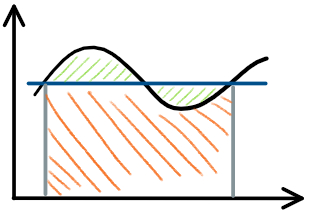
\includegraphics[scale=0.5]{Skizzen/mws_int}
	\end{center}
	\caption{Mittelwertsatz der Integralrechnung}
	\label{plot_MWS_int}
	\end{figure}		
	
	Dann existiert ein $\xi \in [a,b]$ mit 
	\begin{align*}
		\int_a^b f g \dd{x} = f(\xi) \int_a^b g\dd{x}
	\end{align*}
	\textbf{Bemerkung:}
	Für $g = 1$ gilt dann: 
	\begin{align*}
		\int_a^b f \dd{x} = f(\xi) \cdot (b-a)
	\end{align*}
	\textbf{Beweis:} Man setze: $h: [a,b] \rightarrow \mathbb{R},$ $y \mapsto f(y) 
	\cdot \int_a^b g \dd{x}$. $h$ ist stetig und es gilt:
	\begin{align*}
		\inf_{y \in [a,b]} h(y) = & \inf_{y \in [a,b]} \int_a^b f(y) g(x) \dd{x} \\
		\leq & \int_a^b \int_{y \in [a,b]} f(y) g(x) \dd{x} \\
		 \overset{Satz~\ref{vl_11_satz24}}{\le} & \int_a^bf(x)g(x) \dd{x} 
		\overset{Satz~\ref{vl_11_satz24}}{\le}
		\int_a^b \sup_{y \in [a,b]} f(y) g(x) \dd{x} = \sup_{y \in [a,b]} h(y)
	\end{align*}
	D.h wir haben eine stetige Funktion $h$ mit 
	\begin{align*}
		\int_a^b fg\dd{x} \in [\inf_{y \in [a,b]} h(y),  \sup_{y \in [a,b]} h(y)]
	\end{align*}
	\textbf{Bemerkung:} Wir haben bereits gesehen: Polynome sind beliebig oft
	 differenzierbar.
	
}\end{Satz}
%!TEX root = ../gesamt.tex

\cleardoublepage

\section{Differentiation und Integration}

\begin{Bemerkung}{
	Bisher hatten wir stets $\int_a^b f \dd{x}$ mit $ a \leq b$ betrachtet.
	Für $a \geq b$ setze man 
	\begin{align*}
		\int_a^b f \dd{x} := - \int_b^a f \dd{x}
	\end{align*}
}\end{Bemerkung}

\begin{Satz}{\label{vl_12_satz_01}
	Sei $f \in \mathcal{R}_{[a,b]}$. Für $ a \leq x \leq b$ setze man 
	\begin{align*}
		F(x) = \int_a^x f(t) \dd{t}
	\end{align*}
	Dann gilt
	\begin{enumerate}
		\item $F$ ist stetig auf $[a,b]$
		\item Ist $f$ stetig in $x_0 \in [a,b]$, so ist $F$ in $x_0$ differenzierbar 
		und es \linebreak gilt: $F'(x_0) = f(x_0)$
	\end{enumerate}
}\end{Satz}


\begin{proof}~
	\begin{enumerate}
		\item Da $f \in \mathcal{R}_{[a,b]}$, ist $f$ insbesondere beschränkt.
		Das heißt es existiert ein $M \in \mathbb{R}$ mit 
		\begin{align*}
			\forall x \in [a,b]:\abs{f(x)} \leq M
		\end{align*}
		Sei nun $\epsilon > 0$ gegeben. Setze $\delta := \frac{\epsilon}{M}$. 
		Für $x, y \in [a,b]$ mit $\abs{x-y} < \delta$ erhalten wir:
		\begin{align*}
			\abs{F(x) - F(y)} = & \abs{\int_a^x f \dd{t} - \int_a^y f \dd{t} }\\
			= &  \abs{ \left (\int_a^y f\dd{t} + \int_y^x f\dd{t} \right ) - \int_a^yf\dd{t}} \tag{Satz~\ref{vl_11_satz24}-4}\\
			= & \abs{\int_y^x f\dd{t}} \leq \int_y^x \abs{f} \dd{t} \tag{Satz~\ref{vl_11_satz_25}}\\
			\leq & M \cdot \int_y^x 1 \dd{t} = M (x-y) < \epsilon
		\end{align*}
		Da $\epsilon > 0$ beliebig gewählt war, folgt die Aussage
		\item Sei $h \in \mathbb{R}$, so dass $x_0 +h \in [a,b]$.
		Dann gibt es ein $\xi_h$ zwischen $x_0$ und $x_0+h$ mit:
		\begin{align*}
			\frac{F(x_0 + h) - F(x_0)}{h}
			= & \frac{ \int_a^{x_0+h}f(t)\dd{t}- \int_a^{x_0}f(t)\dd{t}}{h} \\
			= & \frac{h}{1} \int_{x_0}^{x_0+h} f(t)\dd{t} \\
			= & \frac{1}{h} f(\xi_h) \cdot \int_{x_0}^{x_0+h} \dd{t} \tag{Satz~\ref{satz:mws_integral}}\\
			= & \frac{1}{h} f(\xi_h) \cdot h
		\end{align*}
		 Damit gilt (wegen der Stetigkeit von $f$ in $x_0$):
		 \begin{align*}
		 \lim\limits_{h \rightarrow 0}{\frac{F(x_0+h)-F(x_0)}{h}} 
			= \lim\limits_{h \rightarrow 0} f(\xi_h) = f(x_0)
		 \end{align*}
	\end{enumerate}
\end{proof}


\begin{Satz}[Hauptsatz der Differential- und Integralrechnung]{\label{vl_12_satz_02}
	Ist $f \in \mathcal{R}_{[a,b]}$ und es gilt $F: [a,b] \rightarrow \mathbb{R}$
	differenzierbar mit $F' = f$. Dann gilt
	\begin{align*}
		\int_a^b f\dd{x} = F(b) - F(a) 
	\end{align*}
}\end{Satz}

\begin{Bemerkung}{
	~\begin{itemize}
		\item Eine Funktion $F$ mit $F'=f$ nennt man eine \emph{Stammfunktion} 
		von $f$
		\item Man schreibt gerne $F(x) \vert_a^b := F(b) -F(a)$
	\end{itemize}
}\end{Bemerkung}

\begin{proof}
	Sei $\epsilon >0 $ gegeben. Man wähle eine Partition $P = \{x_0, \hdots, x_n\}$ 
	mit 
	\begin{align*}
		S(P,f) - s(P,f) < & \epsilon
	\end{align*}
	Weiter existiert aufgrund des Mittelwertsatzes der \\Differential-Rechnung
	(Satz~\ref{vl_07_MWS}) 
	$\xi \in [x_{i-1}, x_i]$ mit 
	\begin{align*}
		F(x_i) - F(x_{i-1}) = &  f(\xi_i) \cdot \Delta x_i
	\end{align*}
	Nach Satz~\ref{kap10_satz19} gilt 
	\begin{align*}
		\epsilon > & \abs{ \int_a^b f \dd{x} - \sum_{i=1}^n f(\xi_i) \Delta x_i} \\
		= & \abs{ \int_a^b f \dd{x} - \sum_{i=1}^n F(x_i) -F(x_{i-1})} \\
		= & \abs{ \int_a^b f \dd{x} - (F(b) -F(a))}
	\end{align*}
	Da $\epsilon > 0$ beliebig gewählt war, folgt die Behauptung.	
\end{proof}

\begin{Bemerkung}{
	\begin{itemize}
	\item[ ]
		\item Sei $f \in \mathcal{R}_{[a,b]}$ Dann bezeichnet man die Funktion 
		\begin{align*}
			\int_a^{\circ} f\dd{x} :  [a,b]  & \rightarrow \mathbb{R} \\
			 t & \mapsto \int_a^b f\dd{x}
		\end{align*}
		\todo{ich bin mir hier nicht sicher ob das nicht t $\mapsto \int_a^x f \dd{t}$ sein müsste}
		als \emph{unbestimmtes Integral} von $f$.
		\item Satz~\ref{vl_12_satz_02}
		sagt also das jede Stammfunktion ein unbestimmtes Integral von $f$ ist 
	\end{itemize}
}\end{Bemerkung}

\begin{Proposition}{
	Sei $F: [a,b] \rightarrow \mathbb{R}$ eine Stammfunktion von $f \in \mathcal{R}
	_{[a,b]}$. Eine Funktion $G: [a,b] \rightarrow \mathbb{R}$ ist genau dann 
	Stammfunktion von $f$, wenn $F-G = konst.$
}\end{Proposition}

\begin{proof}
	 $\Leftarrow$ \\
	Sei $c \in \mathbb{R}$. Dann gilt für $F + c$ 
	\begin{align*}
		(F+ c)' = F' = f
	\end{align*}
	$\Rightarrow$ \\
	Das war eine Folgerung des Mittelwertsatzes der Differentialrechnung 
	(Satz~\ref{vl_07_MWS}).
\end{proof}

\begin{Bemerkung}{
	Oftmals wird ignoriert, dass sobald es eine Stammfunktion $F$ von $f$ gibt, es 
	automatisch unendlich viele gibt. So schreibt man beispielsweise 
	\begin{align*}
		\int f \dd{x} = F
	\end{align*} 
	oder spricht von \glqq der\grqq{} Stammfunktion. Die obige Gleichung ist
	 insofern problematisch, da die rechte Seite (und damit per Definition auch die 
	 linke Seite) nur bis auf eine Konstante bestimmt ist. Oftmals ist daher der 
	 etwas laxe Umgang mit den Begriffen unkritisch.
}\end{Bemerkung}

\begin{Satz}[Partielle Integration]{\label{vl_12_satz_03}
	Seien $F,G: [a,b] \rightarrow \mathbb{R}$ differenzierbar mit 
	\begin{align*}
		F' = f \text{ und } G' = g 
	\end{align*}
	wobei $f,g \in \mathcal{R}_{[a,b]}$. Dann gilt:
	\begin{align*}
		\int_a^b F \cdot g \dd{x} = FG\vert_a^b - \int_a^b f \cdot G \dd{x}
	\end{align*}
}\end{Satz}

\begin{proof}
	\begin{align}\label{vl_12_gl_1}
		\frac{\mathrm{d}}{dt}F(t)\cdot G(t) = & F(t)G(t) + F(t)G'(t) = 
		f(t)G(t) + F(t)g(t)
	\end{align}
	Da $f,g \in \riemann a b$ und $F,G$ differenzierbar (und daher auch in 
	$\riemann a b$), ist die rechte Seite in $\riemann a b$. \\
	Mit Satz~\ref{vl_12_satz_02} haben wir:
	\begin{align*}
		\int_a^b f(t) G(t) + F(t)g(t) \dd{t} = F(b)G(b) -F(a)G(a)
	\end{align*}
	Weiter aufgrund der Linearität des Integrals:
	\begin{align*}
		\int_a^bfG + Fg \dd{t} = \int_a^b fG\dd{t} + \int_a^b Fg\dd{t} \\
		\ref{vl_12_gl_1}-\int_a^b fG\dd{t}
	\end{align*}
	liefert die Behauptung.
\end{proof}

\begin{proof}
	\begin{align*}
		\left( FG|_a^x - \int_a^x f \cdot G \dd{t} \right)' = &
		\left(F(x) \cdot G(x) - F(a) \cdot G(a) - \int_a^x fG \dd{t} \right)' \\
		= & F'(x)G(x) + F(x)G'(x) - f(x)G(x)) \\
		= & f(x)G(x) + F(x)g(x) -f(x)G(x)
	\end{align*}
	Ergo: die rechte Seite ist eine Stammfunktion des Integranden der 
	linken Seite. Damit folgt die Aussage aus Satz~\ref{vl_12_satz_02}.
\end{proof}

\begin{Beispiel}{
	\begin{align*}
		& \int_a^b cos^2(x) \dd{x} & = &  \int_a^b cos(x) \cdot cos(x) \dd{x} \\
		& &  = & \left. cos(x) \cdot sin(x) \right\vert_a^b + 
			\int_a^b sin^2 \dd{x} \\
		& & = & \left. cos(x) \cdot sin(x) \right\vert_a^b + 
			\int_a^b 1 - cos^2(x) \dd{x} \\
		& & = & \left. cos(x) \cdot sin(x) \right\vert_a^b 
			+ \int_a^b 1 \dd{x} \\
		& & & - \int_a^b cos^2(x) \dd{x} 
			 \; \left\vert + \int_a^b cos^2(x) \dd{x} \right. \\
	 \Leftrightarrow 
	 & 2 \int_a^b cos^2(x) \dd{x} & = & \left. cos(x) \cdot sin(x) \right\vert_a^b 
	 	+ \left. x \right\vert_a^b  \left\vert \cdot \frac{1}{2} \right. \\
	 \Leftrightarrow
	& \int_a^b cos^2(x) \dd{x} & = & \frac{1}{2} \cdot 
		\left. \left( cos(x) \cdot sin(x) + x\right) \right\vert_a^b \\
	\text{Ergo: } & \int_a^b cos^2(x) \dd{x} & = & \frac{1}{2} (cos(x) sin(x) 
		\vert_a^b + (b-a))
	\end{align*}
	\begin{align*}
		\int_a^b \ln (x) \dd{x} \text{ wobei } 0 \not\in [a,b] \\
		\int 1 \cdot \ln (x) \dd{x} = & x \cdot \ln (x)\vert_a^b - 
		\int_a^b x \cdot \frac{1}{x} \dd{x} \\
		= & \left. x \cdot \ln (x) \right\vert_a^b - \int_a^b 1 \dd{x} \\
		= & \left. x \cdot \ln (x)\right\vert_a^b - \left. x\right\vert_a^b \\
		= & \left. x \cdot \ln (x)\right\vert_a^b - (b - a)
	\end{align*}
}\end{Beispiel}

\begin{Satz}{\label{vl_12_satz_04}
	Sei $f: [a,b] \rightarrow \mathbb{R}$ stetig und $\phi: [c,d] \rightarrow [a,b]$ 
	stetig differenzierbar. Dann gilt:
	\begin{align*}
		\int_a^b f(\phi(t))\cdot\phi'(t)\dd{t} = \int_{\phi(c)}^{\phi(d)} 
		f(x) \dd{x}
	\end{align*}	 
}\end{Satz}


\begin{proof}
	Sei $F : [a,b] \rightarrow \mathbb{R}$ eine Stammfunktion von $f$. Dann gilt für 
	$t \in [c,d]$:
	\begin{align*}
		\frac{\mathrm{d}}{\mathrm{dt}}F(\phi(t)) = &  F'(\phi(t)) \cdot \phi'(t) \\
		= & f(\phi(t))\cdot \phi'(t) \\
		\text{Ergo: } \int_{\phi(c)}^{\phi{d}} = & \int F(\phi(d))-F(\phi(c)) \\
		= & \int_a^b f(\phi(t)) \phi'(t) \dd{t}
	\end{align*}
\end{proof}

\begin{Bemerkung}{
	\begin{itemize}
		\item[ ]
		\item Die Substitutionsregel lässt sich wie folgt nachrechnen
		\begin{align*}
			\phi'(t)\mathrm{dt} = \frac{\mathrm{d\phi}}{\mathrm{dt}}dt
		\end{align*}
		Dann lässt sich die Substitutionsregel
		\begin{align*}
			\int_c^d f(\phi) \dd{\phi} = \int_{\phi(c)}^{\phi(d)} f(x) \dd{x}
		\end{align*}
	\end{itemize}
}\end{Bemerkung}

\begin{Beispiel}{
	\begin{align*}
		\int_{-r}^r \sqrt{r^2 -x^2} \dd{x} = r \int_{-r}^r 
		\sqrt{1 - \frac{x^2}{r^2}} \dd{x}
	\end{align*}
	Wir wählen $\phi(t) = r \cdot sin(t)$ für $ t \in [\frac{-\pi}{2}, \frac{\pi}{2}]$. 
	Dann gilt mit der Substitutionsregel 
	(man beachte dass $\phi(\frac{-\pi}{2}) = -r 
	$ und $\phi(\frac{\pi}{2}) = r$):
	\begin{align*}
		r \cdot \int_{-r}^r \sqrt{1 - \frac{x^2}{r^2}} \dd{x} = & r 
			\cdot \int_{-\frac{\pi}{2}}^{\frac{\pi}{2}} 
			\sqrt{1 - \frac{\phi^2(t)}{r^2}} \cdot \phi'(t) \dd{t} \\
		= & r \cdot \int_{-\frac{\pi}{2}}^{\frac{\pi}{2}} 
			\sqrt{cos^2(t)} \cdot cos(t) \cdot r\dd{t} \\
		= & r^2 \cdot \int_{\frac{-\pi}{2}}^{\frac{\pi}{2}} \cdot cos^2(t)\dd{t} \\
		= & \frac{r^2}{2} \cdot \pi
	\end{align*}	 
}\end{Beispiel}

\begin{Beispiel}
	\begin{align*}
		\int_a^b \frac{\dd{x}}{1-x^2} \text{ wobei } -1, 1 \notin [a,b]
	\end{align*}
	Vorgehen Partialbruchzerlegung: Man zerlegt den Nennen in seine Linearfaktoren 
	und bestimmt Konstanten $\alpha, \beta \in \mathbb{R}$ mit:
	\begin{align*}
		\frac{1}{1-x^2} = \frac{\alpha}{1+x} + \frac{\beta}{1-x}
	\end{align*}
	Man beachte, dass $(1-x)(1+x) = 1 -x^2$ \\
	Wir multiplizieren die Gleichung mit $(1+x)(1-x)$ und erhalten: 
	\begin{align*}
		1 = \alpha (1 -x) + \beta (1+x) 
		= \alpha + \beta (\beta-\alpha)x (x \in [a,b])
	\end{align*}
	Also: $ \alpha = \beta = \frac{1}{2}$
	Damit gilt:
	\begin{align*}
		\int_a^b \frac{\dd{x}}{1-x^2} = \frac{1}{2} \left( \int_a^b \frac{\dd{x}}{1-x} + \int_a^b \frac{\dd{x}}{1+x} \right)
	\end{align*}
	Nun gilt für $\phi(t) = 1 - t$:
	\begin{align*}
		\int_a^b \frac{\dd{x}}{1-x} = \int_{1-a}^{1-b} \frac{-1 \dd{t}}{1 \phi(t)}
		= - \int_{-a}^{1-b} \frac{\dd{t}}{t} = \left. -\ln(t)\right\vert_a^b
	\end{align*}
	Weiter gilt mit $\phi(t) = t-1$:
	\begin{align*}
		\int_a^b \frac{\dd{x}}{1+x} = \int_{1+a}^{1+b} \frac{\dd{t}}{t} = \left.\ln 
		(t) \right\vert_{1+a}^{1+b}
	\end{align*}
	Ergo:
	\begin{align*}
		\frac{1}{2}(\ln(1+b) - \ln(1-b) - (\ln(1+a) - \ln(1-a))
		= \left. \frac{1}{2} \ln \frac{1+x}{1-x}\right\vert_a^b
	\end{align*}	
\end{Beispiel}



\end{document}
 	
